\documentclass[%
xelatex,
	oneside,		% Single side print
	12pt,			% Font size
	parskip=half,	% Half line skip between paragraphs
%	headsepline,	% Line after header
%	footsepline,	% Line before footer
	abstracton,
	chapterprefix=true% like in standard class "report"
    appendixprefix=true]
{scrbook}
\usepackage[english]{babel}

\usepackage{rwukoma}
\usepackage[pdfusetitle]{hyperref}
\title{Master Thesis}
\author{Viplav Setia}
\usepackage{graphicx}
\usepackage{nomencl}
\makenomenclature
\renewcommand{\nomname}{List of abbreviations, formulas and indexes}
\usepackage{blindtext}
\usepackage{caption}
\usepackage{scrlayer-scrpage}
\pagestyle{scrheadings}
\clearscrheadfoot
\rofoot{\pagemark}
\refoot{\pagemark}
\automark{chapter}
\ohead{\headmark}
\setlength{\nomlabelwidth}{2cm}
\setlength{\nomitemsep}{-\parsep}
\usepackage{hyperref}

\begin{document}

\section*{\Large\normalfont\bfseries Declaration}
	\addcontentsline{toc}{chapter}{Declaration}

I, Viplav Setia, born on 04.04.1995 in New Delhi, India, assure that I have done this work independently. All sources and references used for the completion of this
thesis have been listed and cited accordingly. This thesis work was done in
partial fulfillment of the requirements for the award of the degree of Master of
Science in Mechatronics at Hochschule Ravensburg Weingarten and has not been
used or submitted elsewhere for award of a degree, grade or in any publication. \newline


\rule{5cm}{.4pt}

Viplav Setia \newline
Friedrichshafen, 31 January 2020
\clearpage

		\section*{\Large\normalfont\bfseries Acknowledgement}
		\addcontentsline{toc}{chapter}{Acknowledgement}

I would like to express my heartfelt
gratitude to Prof Dr.-Ing Benedikt Reick and Prof Dr. rer. nat. Markus Pfeil for guiding me through the completion of my Master thesis and for their valuable
suggestions.

I am extremely thankful to ALTEN GmbH and their colleagues who gave me this opportunity and the resources to do this thesis at their office branch in Friedrichshafen. They also supported me with their knowledge,  expertise and created a pleasant working environment, without which it would have been difficult to move forward with this project.

Also, many thanks to my family and friends for their constant encouragement.				
	\clearpage
		\section*{\Large\normalfont\bfseries Abstract}
		\addcontentsline{toc}{chapter}{Abstract}

The automotive industry is changing rapidly to new technologies like electromobility and automated driving. All major companies like Daimler, BMW, Tesla, Bosch, etc. are investing heavily to bring electric cars to the market and develop prototypes for automated driving. To support this change, middleware is required which is used as a means of data exchange between various sensors, control systems and actuators. The focus of this thesis is to test the new versions of the middleware, Robot Operating System(ROS\nomenclature{ROS}{Robot Operating System}), which offers support for embedded and real-time systems. Additionally, a model using the Gazebo robot simulator was developed to explore \nomenclature{ADAS}{Advanced Driver Assistance Systems} Advanced Driver Assistance Systems(ADAS) applications using a camera and a Light Detection and Ranging(LIDAR)\nomenclature{LIDAR}{Light Detection and Ranging} sensor as an example to show the data transfer using ROS 2 for the automotive industry. To test the real-time performance of ROS2, an inverted pendulum demo was used and its simulation was visualized on a Linux system enabled with real-time capabilities. To test the version micro-ROS, a demonstrator was built using a STM32 microcontroller with a Nuttx Real-Time Operating System(RTOS\nomenclature{RTOS}{Real-Time Operating System}) installed to show the data transfer of a pressure sensor. To test the real-time performance for this version, an algorithm was created to test the delay in data transfer with different data sizes. Finally, the results were analyzed and discussed which also helps in suggesting future research scope.
\clearpage

	\addcontentsline{toc}{chapter}{List of abbreviations, formulas and indexes}
	
\rofoot[\pagemark]{\pagemark}
\refoot[\pagemark]{\pagemark}
\printnomenclature
	

	\tableofcontents
	
	


	\chapter{Introduction}

\rofoot[\pagemark]{\pagemark}
\refoot[\pagemark]{\pagemark}

A modern car is a complex assembly of all kinds of sensors, control systems, actuators, drives and other mechanical components. A great amount of data is flowing between different components of a car which needs to be managed and also arrive at the right place at the right time. As shown in the figure below, Intel suggests about 4000 GB of data flow per day will take place in the future.

\begin{center}
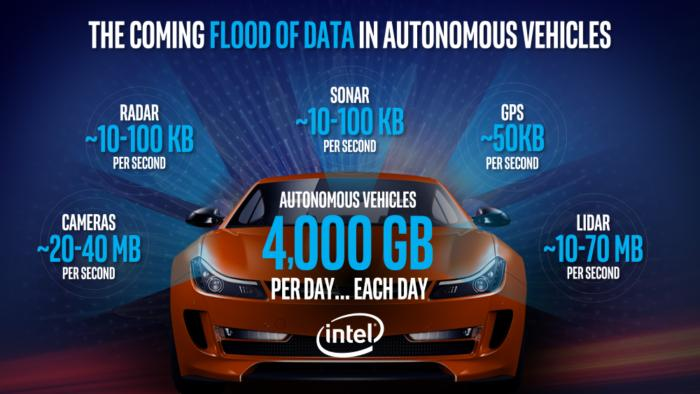
\includegraphics[scale=.5]{fig/autonomous-vehicle-data-intel-100697604-large.jpg}
\captionof{figure}[Data Stats in Autonomous Cars]{Data Stats in Autonomous Cars\cite{datastats}}
\label{fig:datastats}
\end{center}

  
     \section{Motivation}	
For automotive applications, one major challenge is that all systems in the car should be real-time safe, that is, all systems of the car must give a guaranteed response within a specified time constraint. Missing a deadline can have disastrous consequences, such as, failure to apply the brakes at the right time after recognizing a person in front of the car may result in loss of life. 
One such software for communication data management is Robot Operating System(ROS). New versions of ROS, namely, ROS 2 and micro-ROS offer support for real-time systems and embedded boards. The goal of this thesis is to test the real-time capability and robustness of ROS 2 and micro-ROS under different test conditions.
	 \section{Objectives}
\begin{itemize}
  \item Research on state of the art
  \item Apply ROS 2 concepts to explore Automotive ADAS Applications
  \item Set up STM32 microcontroller with RTOS and micro-ROS
  \item Test real-time performance of ROS2 using inverted pendulum demo  
  \item Test real-time performance of micro-ROS
  \item Analyzing results and documentation
\end{itemize}
	 

	 \section{Robot Operating System(ROS)}
	 {\bfseries ROS}
	 
The Robot Operating System (ROS) is a flexible framework for writing robot software. It is a collection of tools, libraries, and conventions that aim to simplify the task of creating complex and robust robot behavior across a wide variety of robotic platforms.\cite{ROS}	
It is an open-source software and is free to use for both research and commercial purposes.
 
But ROS does not guarantee deadlines and requires significant resources like high CPU\nomenclature{CPU}{Central Processing Unit} usage, high memory consumption, etc. Therefore, ROS is not suitable for resource constrained real-time systems.

{\bfseries	 ROS 2}

ROS 2 includes the components of ROS 1 which are great and improves those which are not.	ROS 2 was developed to satisfy new use cases like real-time systems, embedded systems, non-ideal networks, production environments, etc. It also uses new technologies like Data Distribution Service(DDS)\nomenclature{DDS}{Data Distribution Service}. The software is developed and maintained by Open Robotics.
It also offers support for different operating systems such as Linux, macOS, Microsoft Windows and different RTOSs. 
	 \clearpage
{\bfseries	 ROS 2 Distributions}
	 

The ROS 2 Distributions are shown below in descending order of release date. Dashing Diademata is the first long term support version offered by the ROS developers. The work in this thesis is based on the versions Crystal Clemmys and Dashing Diademata. Dashing version release states that it is an improvement over the Crystal version especially for using less memory during runtime which helps in achieving better real-time performance. 

 
 

 
\includegraphics[scale=.112]{fig/eloquent-small.png} \hspace*{1cm}

\includegraphics[scale=.09]{fig/dashing-small.png}\hspace*{1cm}
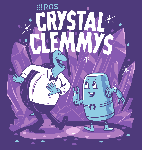
\includegraphics[scale=.48]{fig/crystal-small.png}\hspace*{1cm}

\includegraphics[scale=1]{fig/bouncy-small.png}\hspace*{1cm}

\includegraphics[scale=2]{fig/ardent-small.png}

\captionof{figure}[ROS 2 Distributions]{ROS 2 Distributions\cite{ROS2distro}}
\label{fig:ROS2Distro}

\vspace*{1cm}

{\bfseries	 micro-ROS}
\vspace*{0.5cm}

micro-ROS puts ROS 2 onto microcontrollers, making them first class participants of the ROS 2 environment.\cite{uros}	
It uses a real-time operating system(RTOS), here Nuttx by default, and DDS for eXtremely Resource Constrained Environments(DDS-XRCE)\nomenclature{DDS-XRCE}{DDS for eXtremely Resource Constrained Environments}. In this thesis, ROS 2 Crystal version is used with Nuttx RTOS on a STM32 microcontroller which is a 32-bit microcontroller by STMelectronics. This project is funded by Open Framework for Embedded Robot Applications(OFERA)\nomenclature{OFERA}{Open Framework for Embedded Robot Applications} consortium consisting of Bosch, eProsima, Acutronic Robotics, etc. 

\begin{figure}[ht]
\begin{center}

\includegraphics[scale=.3]{fig/microROS-big-logo.png}
\caption[micro-ROS Logo]{micro-ROS Logo\cite{uroslogo}}
\label{fig:uros}
\end{center}
\end{figure} 
	 
	\chapter{State of the Art}	
		
		
\rofoot[\pagemark]{\pagemark}
\refoot[\pagemark]{\pagemark}
	Real-time applications of ROS 2 have very recently come into the picture by the community. Many people have tested ROS 2 and have identified problems related to real-time performance. Also, the micro-ROS project is still in its infancy stage.
	
The core concepts of ROS 2, micro-ROS, embedded and real-time systems are mentioned in detail in this section. Also, the results of ROS 2 testing by some of the community members are stated.
	\section{ROS 2 Concepts}
	
	\vspace*{0.5cm}
	{\bfseries Node}
	
	
	\vspace*{0.5cm}
An executable/application that runs a program/subprogram that communicate with each other via streaming topics is known as a node.
It is used to communicate with other nodes using ROS client libraries which allow nodes to be written in different programming languages such as C, C++ and python. A robot may contain many nodes to control movement, analyse data, perform an operation like path planning, etc. 

In ROS 2, discovery of nodes is automatic through the underlying middleware. Nodes advertise information to other nodes when they go online, offline and also periodically for new nodes to join and enable communication. ROS 2 design introduces the concept of node lifecycle, which helps to seperate real-time code path from the non real-time tasks. All memory allocations are done during node initialisation.


\vspace*{0.5cm}
	{\bfseries Topic}
	
	
	\vspace*{0.5cm}
	Topics are named buses over which nodes exchange messages. Topics have anonymous publish/subscribe semantics, which decouples the production of information from its consumption. In general, nodes are not aware of who they are communicating with. Instead, nodes that are interested in data subscribe to the relevant topic; nodes that generate data publish to the relevant topic. There can be multiple publishers and subscribers to a topic.\cite{topic}
	
	\vspace*{0.5cm}
	{\bfseries Message}
	
	
	\vspace*{0.5cm}
	Nodes communicate with each other by publishing messages to topics. A message is a simple data structure, comprising typed fields. Standard primitive types (integer, floating point, boolean, etc.) are supported, as are arrays of primitive types. Messages can include arbitrarily nested structures and arrays (much like C structs). msg files are simple text files for specifying the data structure of a message. These files are stored in the msg subdirectory of a package. Nodes can also exchange a request and response message as part of a ROS service call. These request and response messages are defined in srv files.\cite{messages}
	
\begin{center}
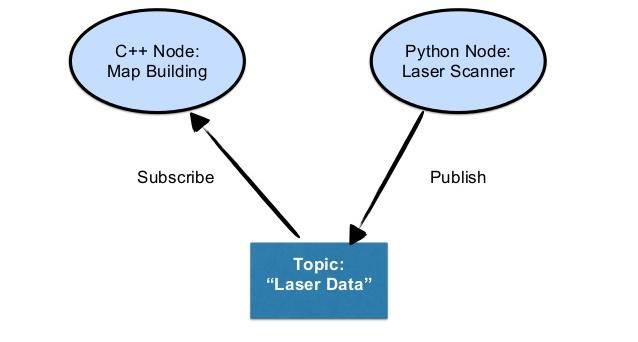
\includegraphics[scale=0.7]{fig/node_topic.jpg}
\captionof{figure}[Working of Nodes, Topics and Messages]{Working of Nodes, Topics and Messages\cite{node_topic}}
\label{fig:node}
\end{center}




	{\bfseries Data Distribution Service(DDS)}
	
	
	\vspace*{0.5cm}
	Data Distribution Service(DDS) is a middleware standard which provides discovery, serialization and transportation to ensure dependable, high performance, interoperable, real-time data exchanges.
	In a distributed system, middleware is the software layer that lies between the operating system and applications. It enables the various components of a system to more easily communicate and share data. It simplifies the development of distributed systems by letting software developers focus on the specific purpose of their applications rather than the mechanics of passing information between applications and systems.\cite{DDS}
		
\begin{center}
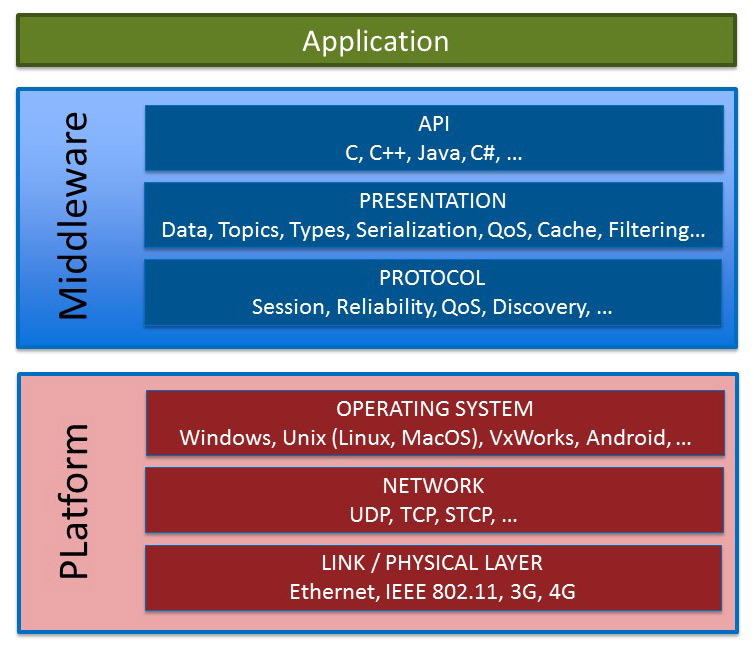
\includegraphics[scale=0.4]{fig/DDS.jpg}
\captionof{figure}[Software Layers in a Distributed System]{Software Layers in a Distributed System\cite{DDS}}
\label{fig:DDS}
\end{center}

\vspace*{0.2cm}
	
	{\bfseries Quality of Service(QoS)\nomenclature{QoS}{Quality of Service}}
	
	
	\vspace*{0.5cm}
	The data can also be shared with flexible Quality of Service (QoS) specifications including reliability, system health (liveliness), and even security. In a real system, not every other end-point needs every item in your local store. DDS is smart about sending just what it needs. If messages don’t always reach their intended destinations, the middleware implements reliability where needed. When systems change, the middleware dynamically figures out where to send which data, and intelligently informs participants of the changes. If the total data size is huge, DDS intelligently filters and sends only the data each end-point really needs. When updates need to be fast, DDS sends multicast messages to update many remote applications at once. As data formats evolve, DDS keeps track of the versions used by various parts of the system and automatically translates. For security-critical applications, DDS controls access, enforces data flow paths, and encrypts data on-the-fly.\cite{DDS}
	
\vspace*{0.2cm}
	
The base QoS profile currently includes settings for the following policies:
\begin{itemize}

\item {\bfseries History}
\begin{itemize}
\item Keep last: only store up to N samples, configurable via the queue depth option.

\item Keep all: store all samples, subject to the configured resource limits of the underlying middleware.
\end{itemize}
\item {\bfseries Depth}
\begin{itemize}
\item Size of the queue: only honored if used together with “keep last”.
\end{itemize}
\item {\bfseries Reliability}
\begin{itemize}
\item Best effort: attempt to deliver samples, but may lose them if the network is not robust.

\item Reliable: guarantee that samples are delivered, may retry multiple times.
\end{itemize}
\item {\bfseries Durability}
\begin{itemize}
\item Transient local: the publisher becomes responsible for persisting samples for “late-joining” subscribers.

\item Volatile: no attempt is made to persist samples.\cite{qos}
\end{itemize}
\end{itemize}

ROS 2, by default, has QoS set to reliable, keep last history and volatile durability. In this thesis, only default QoS settings have been used as ROS 2 Crystal package was installed as a binary package which can be readily used. We can only modify these settings through configuration files of DDS middleware and then installing ROS 2 packages by source. ROS 2 Dashing provides an easier way of changing QoS settings in the source code of the application via Node Options package.
\clearpage


	\section{ROS 1 vs ROS 2}	
	\vspace*{0.5cm}
			\begin{figure}[ht]
\begin{center}
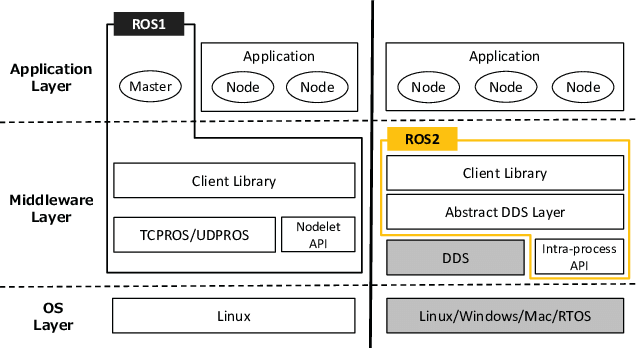
\includegraphics[scale=0.5]{fig/ros1_vs_ros2.jpg}
\caption[ROS 1 vs ROS 2 Architecture]{ROS 1 vs ROS 2 Architecture\cite{rosvsros2}}
\label{fig:rosvsros2}
\end{center}
\end{figure} 

\begin{itemize}
\item {\bfseries Application Layer}


\vspace*{0.5cm}
ROS 2 moves towards a distributed discovery mechanism where nodes advertise information to other nodes. ROS 1 has a centralized discovery mechanism where a master node is required to establish communication between nodes.
\vspace*{0.5cm}
\item {\bfseries Middleware Layer}


\vspace*{0.5cm}
ROS 2 uses DDS standard through which discovery, QoS policies, serialization, and transport is provided which also offers real-time support. ROS 2 also requires new versions of client libraries like C++11 and C++14 and Python 3.5 at least. ROS 1 uses a custom transport protocol, centralized discovery, custom serialization format, and uses C++3 and Python 2 versions.
\vspace*{0.5cm}
\item {\bfseries OS Layer}


\vspace*{0.5cm}
ROS 2 is supported on Linux, Windows 10, macOS and offers the possibilty to run it on a RTOS, whereas ROS 1 is only supported on Linux.
\vspace*{0.5cm}
\end{itemize}

	\section{micro-ROS Architecture}
		\vspace*{0.5cm}
\begin{center}
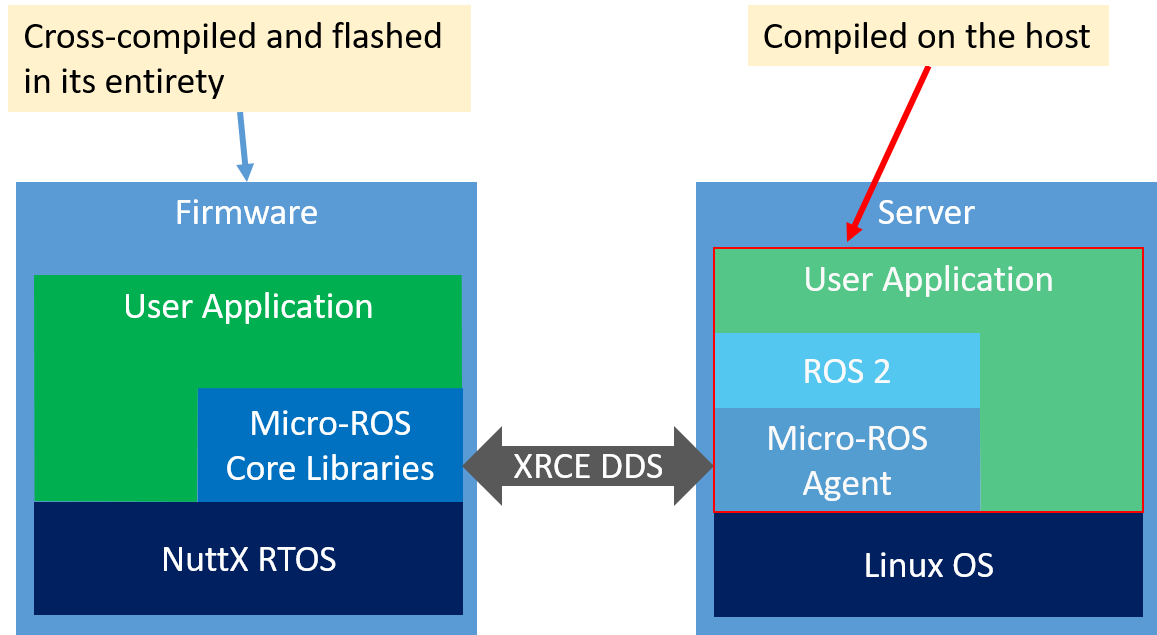
\includegraphics[scale=0.4]{fig/uros_arc.jpg}
\captionof{figure}[micro-ROS Architecture]{micro-ROS Architecture\cite{urosarc}}
\label{fig:urosarc}
\end{center}

 
 
 {\bfseries Firmware/Client}
 
 
 \vspace*{0.5cm}
 The firmware or client is the software cross-compiled(compiled on a different system than the target system) on the host - Linux and flashed onto the target - embedded microcontroller. The micro-ROS software uses Nuttx RTOS by default as its operating system. Nuttx can be configured to run different communication protocols and to run micro-ROS applications. Nuttx has a small footprint and is governed by the standards POSIX(Portable Operating System Interface)\nomenclature{POSIX}{Portable Operating System Interface} and ANSI(American National Standards Institute)\nomenclature{ANSI}{American National Standards Institute}. After enabling micro-ROS and related communication settings in the Nuttx configuration, the user can run the micro-ROS nodes on the microcontroller which can be accessed by Linux through Universal Serial Bus(USB)\nomenclature{USB}{Universal Serial Bus}. The firmware communicates with the host through the DDS-XRCE and connects to the agent running on the host.
 \vspace*{0.5cm}
 
 {\bfseries Agent/Server}
 
 
 \vspace*{0.5cm}
 The agent acts as a server for the clients and communicates with the microcontrollers. It runs on Linux and then can be used to connect with other ROS 2 nodes using the base ROS 2 versions.
 
 
  \vspace*{0.5cm}
  
  {\bfseries Real-Time Executor}
  \vspace*{0.5cm}
  
  
Robot applications require deterministic(predictable) execution of callbacks under all conditions and time constraints. Since the messages are buffered in DDS, ROS 2  introduces the concept of Executor, to support execution management (prioritization of callbacks).
The Logical Execution Time(LET)\nomenclature{LET}{Logical Execution Time} is a known concept in automotive domain to simplify synchronization in process scheduling. If refers to the concept to schedule multiple ready tasks in such a way, that first all input data is read for all tasks, and then all tasks are executed.\cite{let}

This 2 step approach of the LET Executor guarantees a deterministic execution of callbacks.
 
	\section{Hardware and Communication Protocols Used}
	
	\vspace*{0.5cm}
	{\bfseries STM32 Microcontroller}
	
	
	\vspace*{0.5cm}
A Microcontroller Unit(MCU)\nomenclature{MCU}{Microcontroller Unit}	is a compact, integrated circuit which includes input/output peripherals, memory and a processor on a single chip. It is designed to govern a specific operation and is commonly found in automobiles, robots, mobile devices, vending machines, etc. In this thesis work, 32-bit MCUs have been used from the STM family of microcontroller boards. Two development boards, Olimex STM32-E407 and Waveshare STM32-Open407I-C, having similar architectures have been used for testing.

\begin{center}
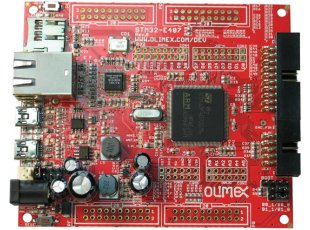
\includegraphics[scale=0.5]{fig/STM32-E407.jpg}\hspace*{1cm}
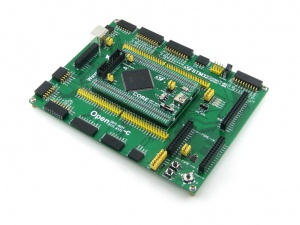
\includegraphics[scale=0.6]{fig/Open407I-C.jpg}


\captionof{figure}[STM32 Development Boards]{STM32 Development Boards\cite{olimex}\cite{waveshare}}
\label{fig:stm32}
\end{center}
\vspace*{0.5cm}	

{\bfseries Communication Protocols}
	
	
\vspace*{0.5cm}
Following are the communication protocols used in testing of micro-ROS:
\begin{itemize}
\item {\bfseries Internet Protocol(IP)}\nomenclature{IP}{Internet Protocol} - It is the main communication protocol to transmit datagrams across network boundaries through IP addresses. The MCU is assigned an IP address and a local area network is setup through ethernet wires between the computer and the MCUs to enable the micro-ROS Client Agent connection. User Datagram Protocol(UDP),\nomenclature{UDP}{User Datagram Protocol} part of IP suite, supported by micro-ROS is used in this thesis work.
\item {\bfseries USB-Serial} - PL2303 peripheral device is used to connect the board’s UART(Universal Asynchronous Receiver-Transmitter)\nomenclature{UART}{Universal Asynchronous Receiver-Transmitter} pins to the USB of the computer to enable communication via USB wire. However, the speed of data transfer is slower than IP because of the PL2303 driver used.
\item {\bfseries Inter-Integrated Circuit(I2C)}\nomenclature{I2C}{Inter-Integrated Circuit} - is a multi-wire serial bus protocol to allow communication between small chips(slaves) with bigger chips(master). In this thesis work, a demonstrator for micro-ROS using a digital air pressure sensor was built which uses I2C protocol between the sensor and the MCU.
\end{itemize}

	
	\section{Real-Time Systems}
	
	
	\vspace*{0.5cm}	
Real-time systems should produce reproducable and correct computations at the correct time and be predictable even in a worst case scenario. Failure to respond within a set desired time(deadline) can cause damage to life or other resources. These systems have to be designed according to the dynamics of the physical process. They are often part of an embedded system and are employed in airplane sytems, automotive systems, satellites, power stations, and other critical applications. These systems are usually resource-constrained and still should offer low latencies. Jitter is the variation in the periodic loop time.
	
	\begin{center}
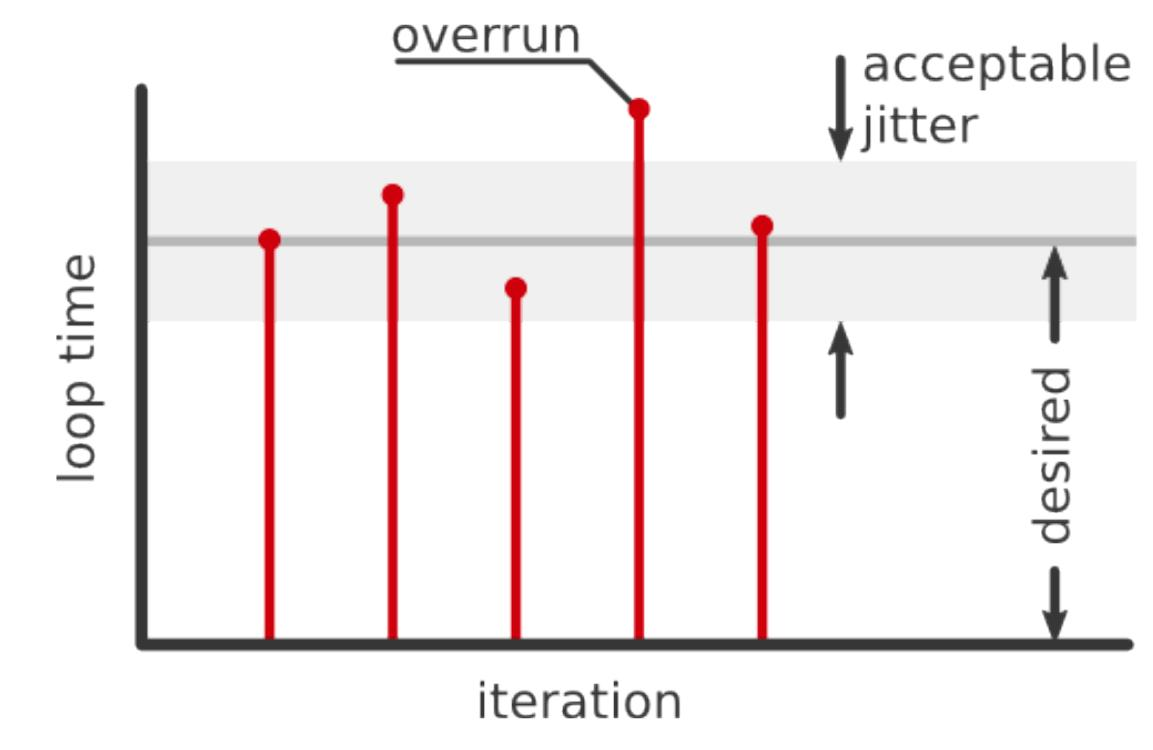
\includegraphics[scale=0.4]{fig/deadline.jpg}
\captionof{figure}[Deadline and Jitter in Real-Time Systems]{Deadline and Jitter in Real-Time Systems\cite{deadline}}
\label{fig:deadline}
\end{center}
	The different types of real-time systems are:
	\begin{itemize}
\item	{\bfseries Soft} - The result can still be used after the deadline. For example, audio/video playback failure will only cause irritation to the user.
\item	{\bfseries	Firm} - The result does not have utility after the deadline. For example, in an automated manufacturing facility with high production rate, if the part does not arrive in time for a process to take place and the part is skipped or the machines stop, then it can cause financial losses to the facility.
\item	{\bfseries	Hard} - Missing a deadline can be catastrophic and can cause serious damage to life and property. For example, the landing gear of an airplane fails to deploy in time during landing.
	\end{itemize}
	
	
	\section{Research by ROS Community}
\vspace*{0.5cm}
\begin{itemize}
\item {\bfseries Inverted Pendulum demo} - The unstable arrangement of an inverted-pendulum is used as a means to test  the real-time performance of ROS 2. A simulation is performed with ROS 2 where, the pendulum is balanced by a motor and a moving cart at the base. The motor command and sensor feedback are configured as ROS 2 messages and these are updated with a loop time of 1 msec. Linux preemtible kernel is used which offers real-time capability. High scheduling priority is given to the node and memory allocations are done during initialisation of the node. Dynamic memory allocations are blocked as they are not real-time safe. J. Kay and A.R. Tsouroukdissian have implemented this package with ROS 2 Alpha release. They also mention that DDS can be fine tuned for better real-time performance. Their goal was to get less than 3\%(30 microsecs) jitter. Without any stress to the system, the maximum jitter was 3.51\% , minimum was 0.16\%, and mean was 0.46\% but with stress on the processor, the maximum jitter was 25.8\% , minimum was 0.14\%, and mean was 0.38\%. Also, 3 instances of overrun(loop time out of acceptable jitter range) were observed.
	\begin{center}
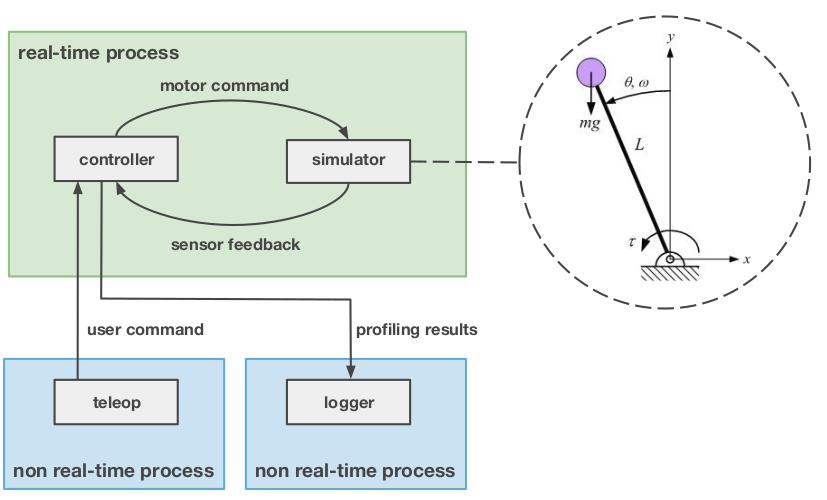
\includegraphics[scale=0.5]{fig/inverted.jpg}

\captionof{figure}[Inverted Pendulum Setup]{Inverted Pendulum Setup\cite{deadline}}
\label{fig:inverpen}
\end{center}
\item {\bfseries Non-deterministic scheduling by ROS 2 Standard Executor} - In a recent study by researchers at Bosch (for more details, see\cite{ingo}), it has been found that the ROS 2 C++ Executor in version Crystal Clemmys has some undesired properties for real-time scheduling. They are:
\begin{itemize}
\item The Executor gives highest priority to timers and therefore messages from the DDS queue are not processed in overloaded situations.
\item Non-preemptive round-robin scheduling of non-timer handles/entities(subscriptions, services,clients) leads to priority inversion, lower priority callbacks may block higher priority callbacks leading to high processing time. Also, this problem is further aggravated as only one message per handle is considered, even when multiple messages of the same topic are available, only one instance is processed by the Executor which causes backlog and hence, priority inversion. 
\end{itemize} 
These shortcomings led to the development of the LET Executor in micro-ROS to allow for deterministic execution.
\item {\bfseries High CPU Overhead by ROS 2 Executor} - In a study by Nobleo Technology (see \cite{nobleo}), it has been concluded that the ROS 2 SingleThreadedExecutor uses a lot of CPU power and generates overhead (unnecessary computation, memory allocations, etc.). ROS 2 Executor needs to be optimised otherwise normal ROS 2 cannot function properly on ARM A-class embedded boards. Based on the discussions between the ROS developers and the community, the Executor is undergoing some design changes to improve its performance. Some changes are planned for the next ROS 2 release Foxy due in May, 2020.
\end{itemize}


	\chapter{ADAS Applications using ROS 2}
		
\rofoot[\pagemark]{\pagemark}
\refoot[\pagemark]{\pagemark}
This is an open source project using License Apache 2.0 to understand simple ADAS applications using ROS 2 Crystal and Gazebo Simulator. You can drive around the robot in the simulator and have Lane Detection and Auto Brake when object is detected. To run this simulator, please refer to the instructions given in my Github repository, see link - \href{https://github.com/Viplav04/ADAS-ROS2-Gazebo-Simulator}{ADAS Simulator using ROS 2 and Gazebo}\cite{ADASsim}
	\begin{center}
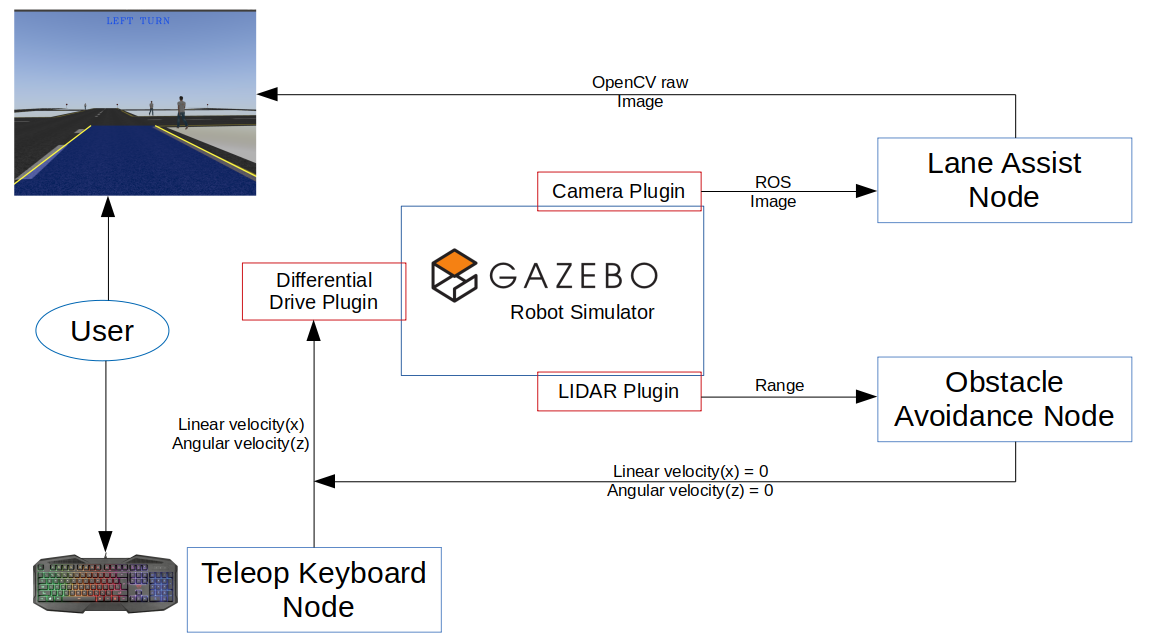
\includegraphics[scale=0.26]{fig/ros2adas.png}
\captionof{figure}[ADAS Simulator using ROS 2 and Gazebo]{ADAS Simulator using ROS 2 and Gazebo}
\label{fig:ADAS}

\end{center}

ROS 2 and Gazebo are both developed by Open Robotics. There are various plugins available to convert Gazebo to ROS 2 data. I have used a camera sensor and a laser sensor in the simulator with my robot which also has a differential drive and can be driven around with the help of a keyboard. The algorithms are developed using C++ language.

Firstly, a world file is created in the Gazebo Simulator to add roads and humans. The robot is modified from the differential drive demo already available in ROS 2 Gazebo tutorials and a camera and laser sensor is added. This setup consists of 3 nodes as explained below.
		\section{Lane Detection using Camera}
	\vspace*{0.5cm}
	Important steps to do lane detection for an image are : 
	\begin{itemize}
\item	The input image subscribed from Gazebo simulator is a ROS message because of the camera plugin. First, it has to be encoded to a raw image to use Open Computer Vision(OpenCV)\nomenclature{OpenCV}{Open Computer Vision} libraries. The raw image is then converted to a grayscale image.
\begin{center}
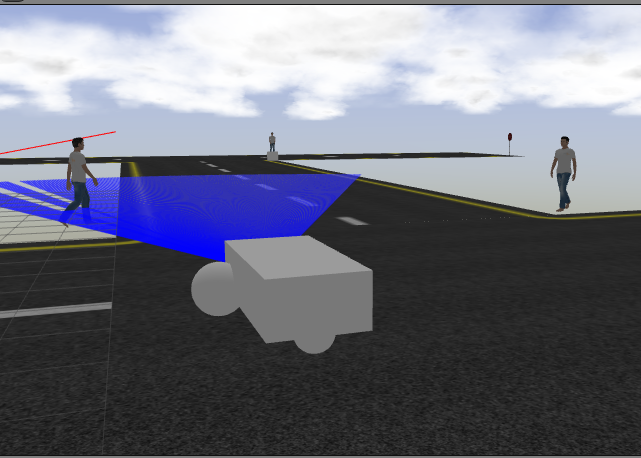
\includegraphics[scale=0.4]{fig/canny1.png}
\captionof{figure}[Gazebo Environment]{Gazebo Environment}
\label{fig:gazebo}
\end{center}
\item Canny Edge Detector from OpenCV libraries is applied to the greyscale image to detect edges.
	\begin{center}
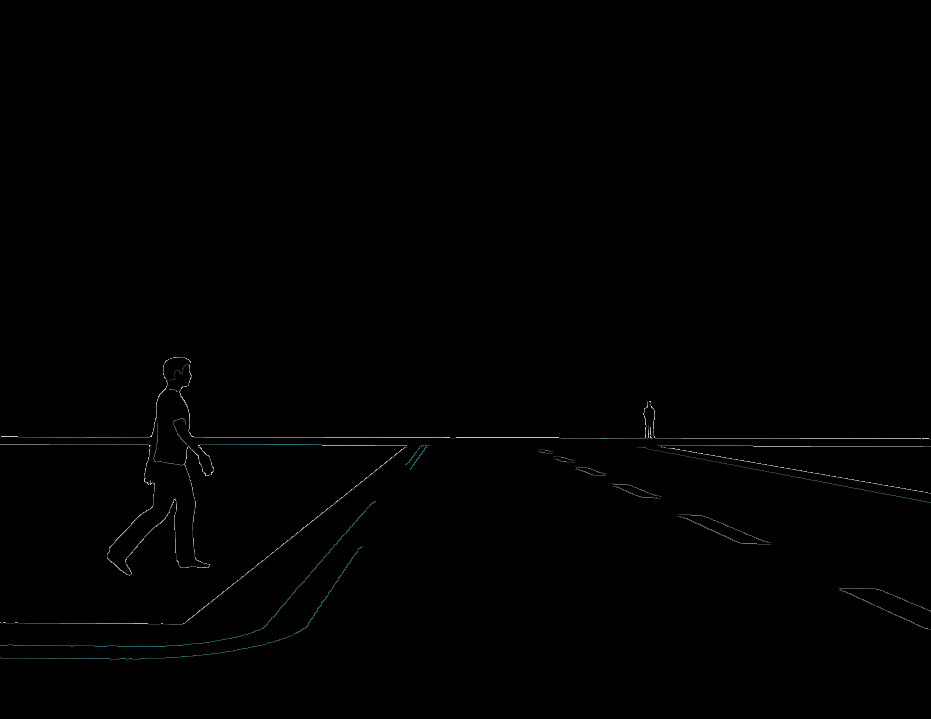
\includegraphics[scale=0.3]{fig/canny.png}
\captionof{figure}[Canny Edge Detection]{Canny Edge Detection}
\label{fig:canny}
\end{center}
\item An image mask is created according to the input image size which filters out the edges in the bottom half of the screen to show only the bottom edges. Then, Hough Transform from OpenCV libraries is applied to the resulting image which detects straight lines. The straight lines are then superimposed to the original raw image.
\begin{center}
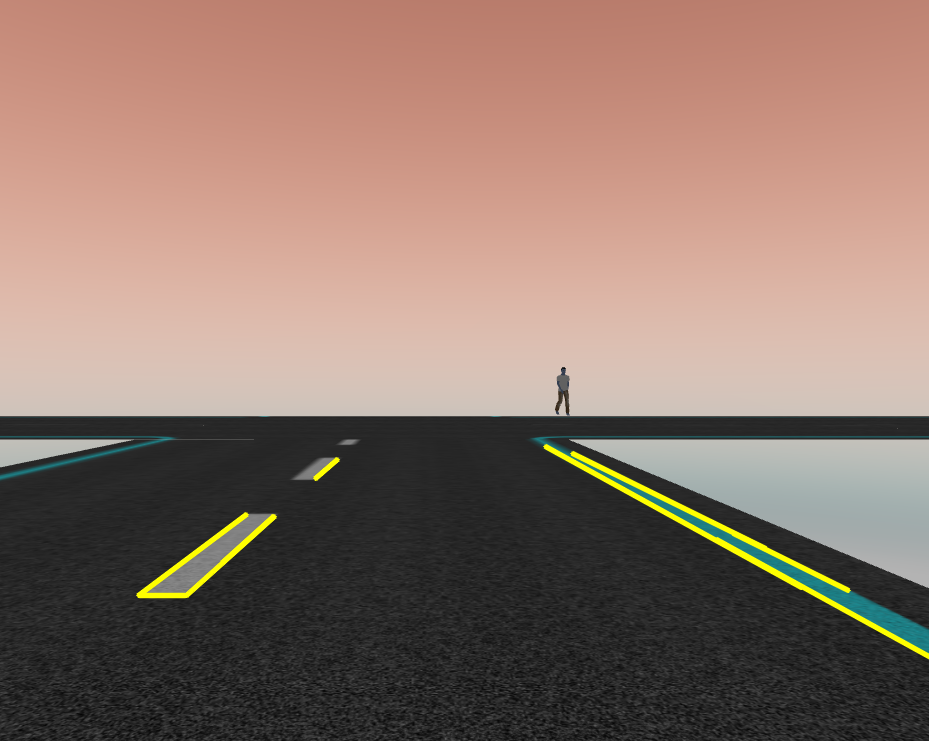
\includegraphics[scale=0.3]{fig/hough.png}
\captionof{figure}[Line Detection using Hough Transform]{Line Detection using Hough Transform}
\label{fig:hough}
\end{center}
\item The lines detected are further optimised and a box is drawn connecting the two lines to display the lane. Also. turning advice to stay in the lane is printed onto the image calculating the direction in which the robot is heading.
\begin{center}
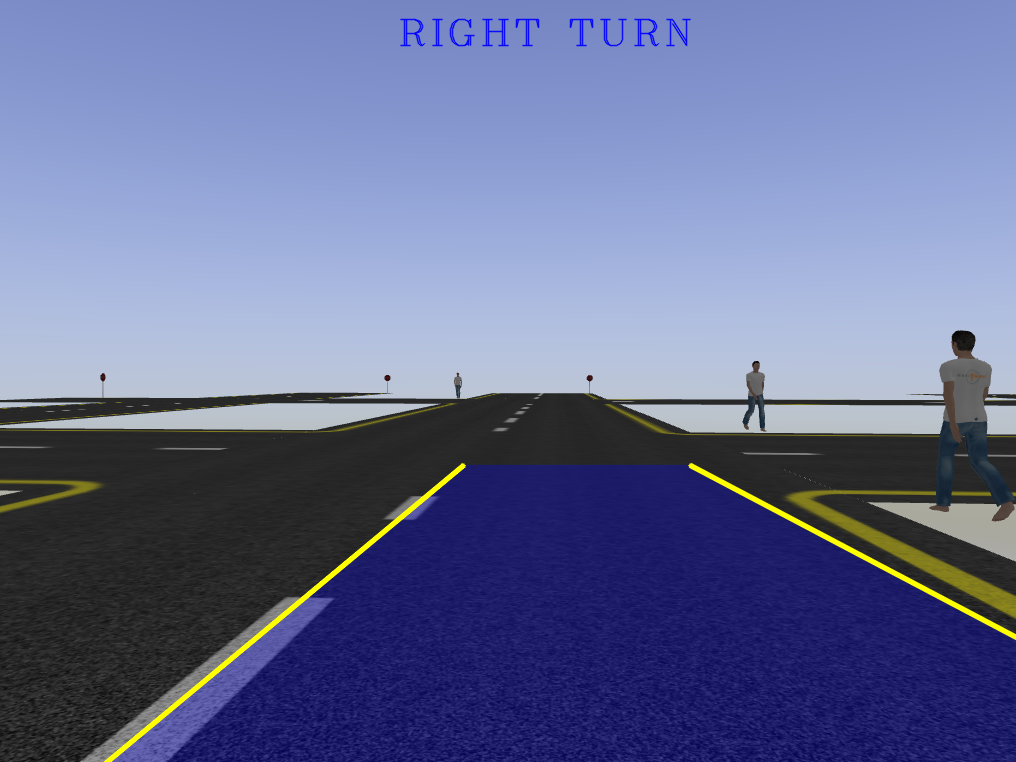
\includegraphics[scale=0.3]{fig/finaladas.png}
\captionof{figure}[Lane Detection]{Lane Detection}
\label{fig:lane}
\end{center}
	\end{itemize}
		
				\section{Driver Control using Keyboard}	
	\vspace*{0.5cm}
The robot has 3 wheels and a differntial drive to enable turning. ROS 2 offers a built-in teleop\textunderscore twist\textunderscore keyboard package to send messages to the robot from the keyboard. The messages are already available in ROS 2 known as Twist messages. The differential drive plugin with Gazebo simulator can be enabled by modifying the robot model file in Gazebo. 	

		\section{Auto Stop using LIDAR}
		\vspace*{0.5cm}
		
The laser sensor data gives out the minimum range of any object in its field. Range messages are already available in ROS 2. Then, an algorithm is applied to the incoming data and a condition is added. When the object is within a range of 4m, this node publishes a new Twist message to the robot telling it to stop. Also, it sends a "STOP, Reverse or Change direction" comment to the user and also prints out in the image running the in the lane detection node. The laser data can be visualized in the RViz package of ROS 2.
			\begin{center}
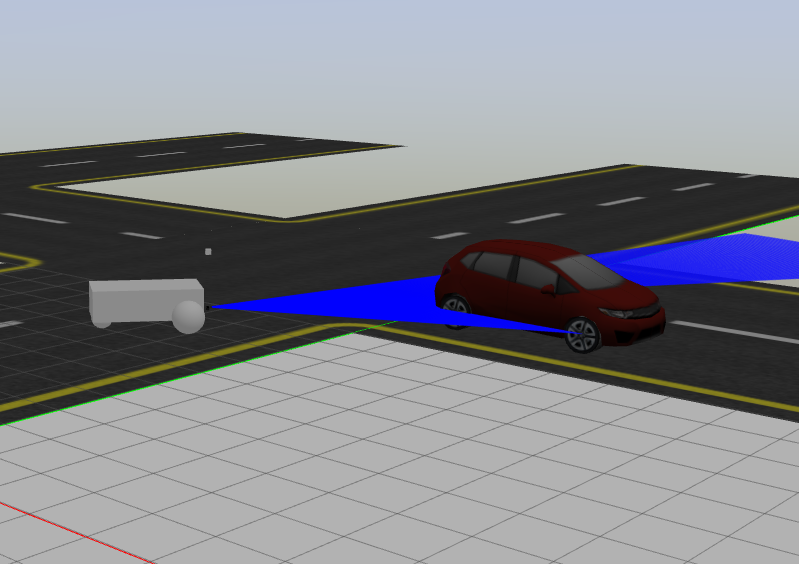
\includegraphics[scale=0.3]{fig/laser.png}
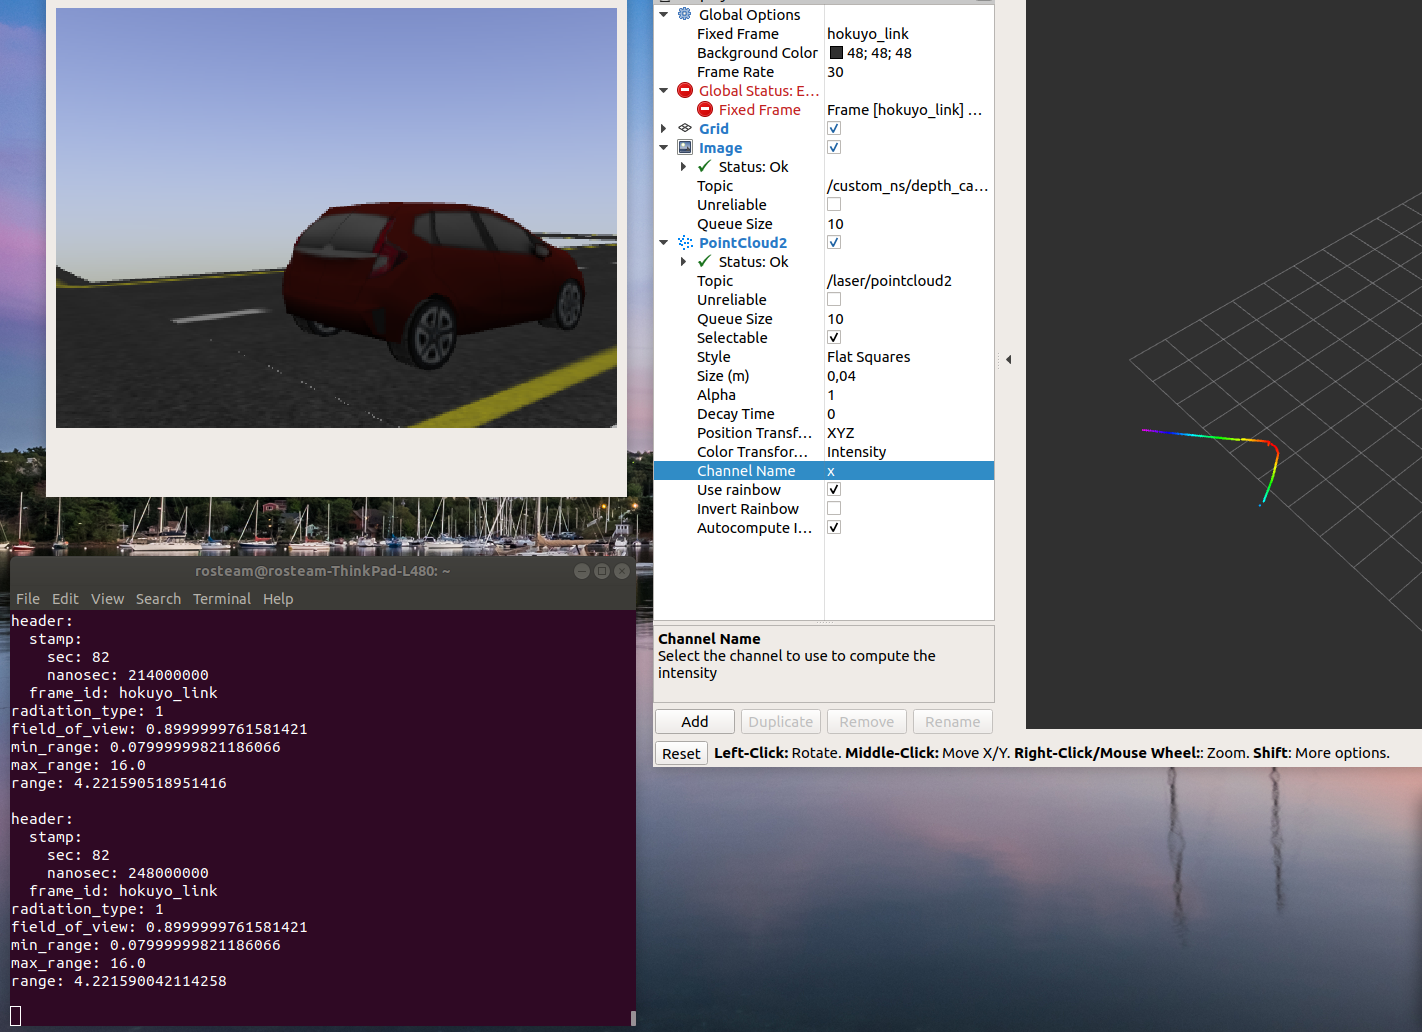
\includegraphics[scale=0.17]{fig/laser2.png}
\captionof{figure}[Laser and Camera Data Visualisation]{Laser and Camera Data Visualisation}
\label{fig:laser}
\end{center}
			\begin{center}
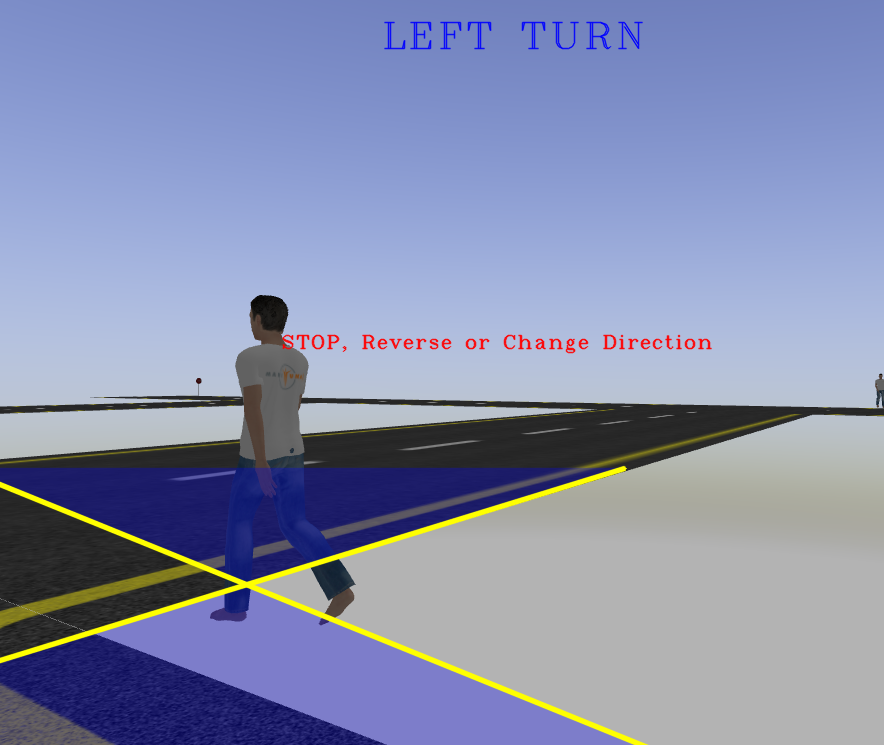
\includegraphics[scale=0.3]{fig/final2adas.png}
\captionof{figure}[Auto Stop Feature]{Auto Stop Feature}
\label{fig:lane1}
\end{center}
This project helps us to understand ROS 2 concepts and also explore its versatile libraries. Along with the Gazebo simulator, different kinds of robot applications can be tested and simulated in the worst case scenarios. 

Different types of data can be accessed in a single node with multiple publishers or subscribers. Also, nodes can interact and discover themselves automatically, the user just has to source the ROS 2 software and launch the created nodes in different terminals in Linux.
	\chapter{Test Setup}
		
\rofoot[\pagemark]{\pagemark}
\refoot[\pagemark]{\pagemark}
The main part of this thesis work was to set up the micro-ROS environment on the STM32 Embedded board and test it, but ROS 2 testing packages were also available and therefore the standard ROS 2 stack was also tested.
	
\section{Testing ROS 2}
\vspace*{0.5cm}
The testing of ROS 2 is based on the inverted pendulum demo. The demo is different for ROS 2 Crystal and Dashing versions. ROS 2 Crystal has an in-built demo as part of its package. There is another version of this demo in development for ROS 2 Dashing and newer versions. We can also visualize the inverted  pendulum simulation in RViz.
			\begin{center}
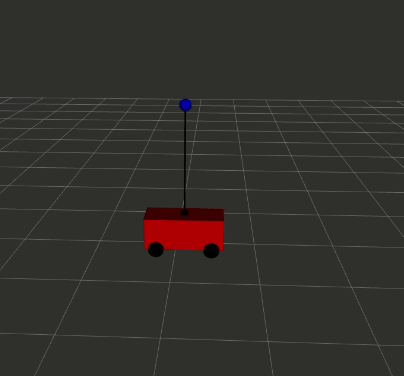
\includegraphics[scale=0.51]{fig/invertedpendulum.png}
\captionof{figure}[Inverted Pendulum Simulation in RViz]{Inverted Pendulum Simulation in RViz}
\label{fig:invertedpendulum}
\end{center}

	\subsection{Components}
	\vspace*{0.5cm}
	\begin{itemize}
	\item Linux system with Ubuntu 18.04 installed
	\item Linux real-time patch and RT-PREEMPT kernel which offers real-time testing capability
	\item ROS 2 Crystal and Dashing versions installed
	\item Inverted Pendulum demo for Dashing (see \href{https://github.com/ros2-realtime-demo/pendulum}{ROS2-realtime-demo}\cite{rtpendulum}) 
	\end{itemize}
	\subsection{Procedure}	
\vspace*{0.5cm}
{\bfseries To set real-time settings in Linux kernel} :
\begin{itemize}
\item Ubuntu 18.04 has SecureBoot security feature. It only allows signed kernels to be installed. Therefore, the real-time kernel after installation has to be signed. To do this, see \href{https://askubuntu.com/questions/1081472/vmlinuz-4-18-12-041812-generic-has-invalid-signature}{Signing a kernel}.
\item To set memory locking and high real-time scheduling priority, the following lines are added to the file /etc/security/limits.conf :
\begin{itemize}
\item "<user>  - memlock limit-in-kilobytes(kB)" (-1 for unlimited, we use 1000 kB\nomenclature{kB}{Kilobyte})
\item "<user>  - rtprio 75" , warning : do not set priority to 99 as it may interfere with important computer processes.
\item The user has to logout and login again to see the changes. To run as a root user, type "sudo su" in a terminal and enter the password to have access to real-time settings and then launch the pendulum demo as root.
\end{itemize}
\end{itemize}

{\bfseries For ROS 2 Crystal} :
\begin{itemize}
\item The ROS 2 Crystal setup.bash file is sourced in a terminal and "pendulum\textunderscore demo>output.txt" command is launched as root user. The node writes the output to the text file.
\item This node sends a 1000 messages for both the motor controller and feedback sensor with an update rate of 1 msec. The process was repeated 5 times and the average values were calculated.
\item Then in another terminal, "stress --cpu 100" command was launched and also many applications were launched in the computer to put stress on the CPU and memory. Then again the pendulum demo was launched 5 times and observations were recorded.
\end{itemize}
{\bfseries For ROS 2 Dashing} :
\begin{itemize}
\item The pendulum demo package is downloaded in a pendulum\textunderscore ws folder and the environment is built. To run the demo, see the link mentioned above for the inverted pendulum demo for Dashing. We lock 1000 kB of memory for this node.
\item This is a continuous simulation. In another terminal, after sourcing the ROS 2 Dashing environment and pendulum environment, "ros2 topic list" command is run. If the demo is enabled with "--pub-stats" as in the instructions, we should see controller and driver statistics topics. They can be launched by command "ros2 topic echo /topic\textunderscore name ". Then in another terminal, "stress --cpu 100" command was launched.
\item The values were recorded every minute and the simulation was allowed to run for 10 minutes.
\end{itemize}
\section{Testing micro-ROS}
\vspace*{0.5cm}
This testing has been done with micro-ROS Crystal version. Dashing version is still not officially released and I had installation issues with it.
	\subsection{Components}
	\vspace*{0.5cm}
	\begin{itemize}
	\item Linux OS with Ubuntu 18.04 and micro-ROS and Nuttx repositories installed
	\item Olimex STM32-E407 Embedded Board
	\item Waveshare STM32-Open407C Embedded Board
	\item USB to TTL UART PL-2303 converter cable
	\item Waveshare UART TTL to Ethernet Converter DP83848
	\item Ethernet cables
	\item UART cables
	\item BMP180 Pressure Sensor
	\item Olimex JTAG USB OCD ARM Debugger(ARM-USB-OCD-H)
	\item micro-USB cables
	\end{itemize}
	\subsection{Procedure}	
	\vspace*{0.5cm}
	\begin{enumerate}
	\item First, install micro-ROS and Nuttx repositories following instructions in this link - \href{https://micro-ros.github.io/docs/tutorials/basic/getting_started/}{micro-ROS Installation}\cite{urosinstall}.
	\item In this setup, 2 boards with similar architectures were used. Waveshare board was made to work on a serial transport connection and the Olimex board with ethernet (UDP). There is a configuration file in directory "~/uros\textunderscore ws/firmware/mcu\textunderscore ws/uros/rmw\textunderscore microxrcedds/rmw\textunderscore microxrcedds\textunderscore c/\linebreak
	rmw\textunderscore microxrcedds.config" where the type of transport and IP address can be changed.
	\item The most time consuming step is to configure Nuttx to work with micro-ROS, pressure sensor, USB console, Ethernet, Debugging, etc. 
	
	This cannot be explained in brief, but the user can refer to these videos - \href{https://www.youtube.com/channel/UC0QciIlcUnjJkL5yJJBmluw/videos}{Nuttx Channel}\cite{Nuttxchannel}. 
	
	You can also find my configuration file at this link - \href{https://github.com/Viplav04/NuttX/tree/master/configs/olimex-stm32-e407/uros}{micro-ROS Configuration File}\cite{olimexconfigfile}.
	\item After configuring Nuttx, the firware needs to be flashed onto the board. Connect the olimex board to the JTAG debugger and micro-USB cable to access the board's operating system (console). 
	
				\begin{center}
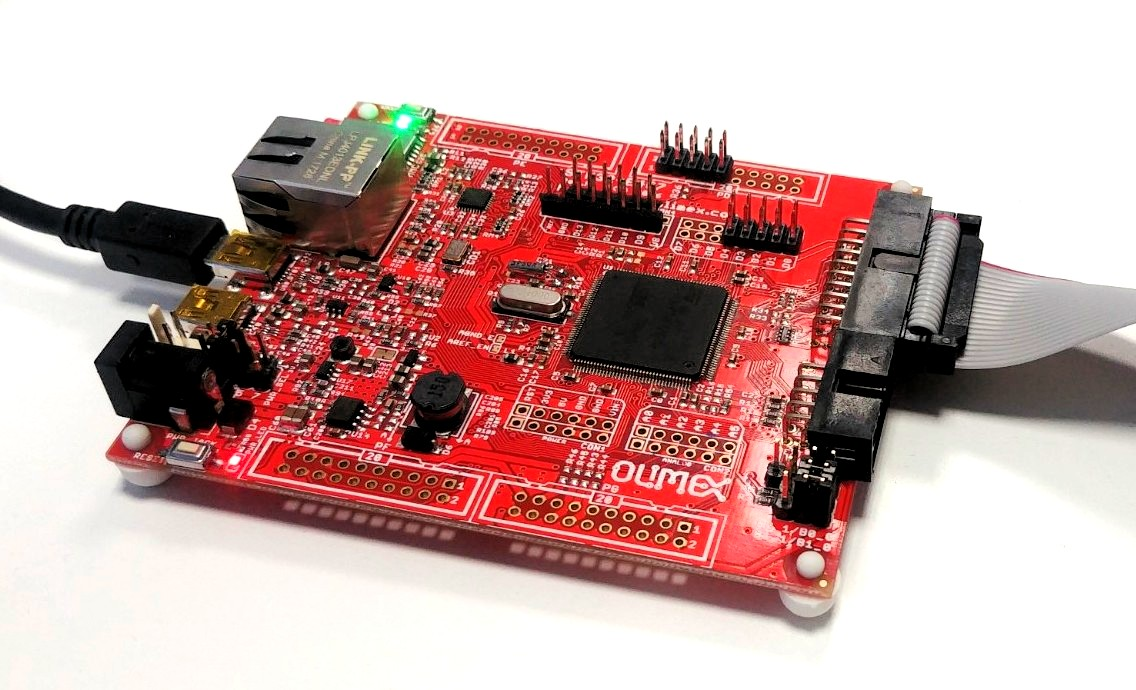
\includegraphics[scale=0.2]{fig/olimexnshusb.jpg}
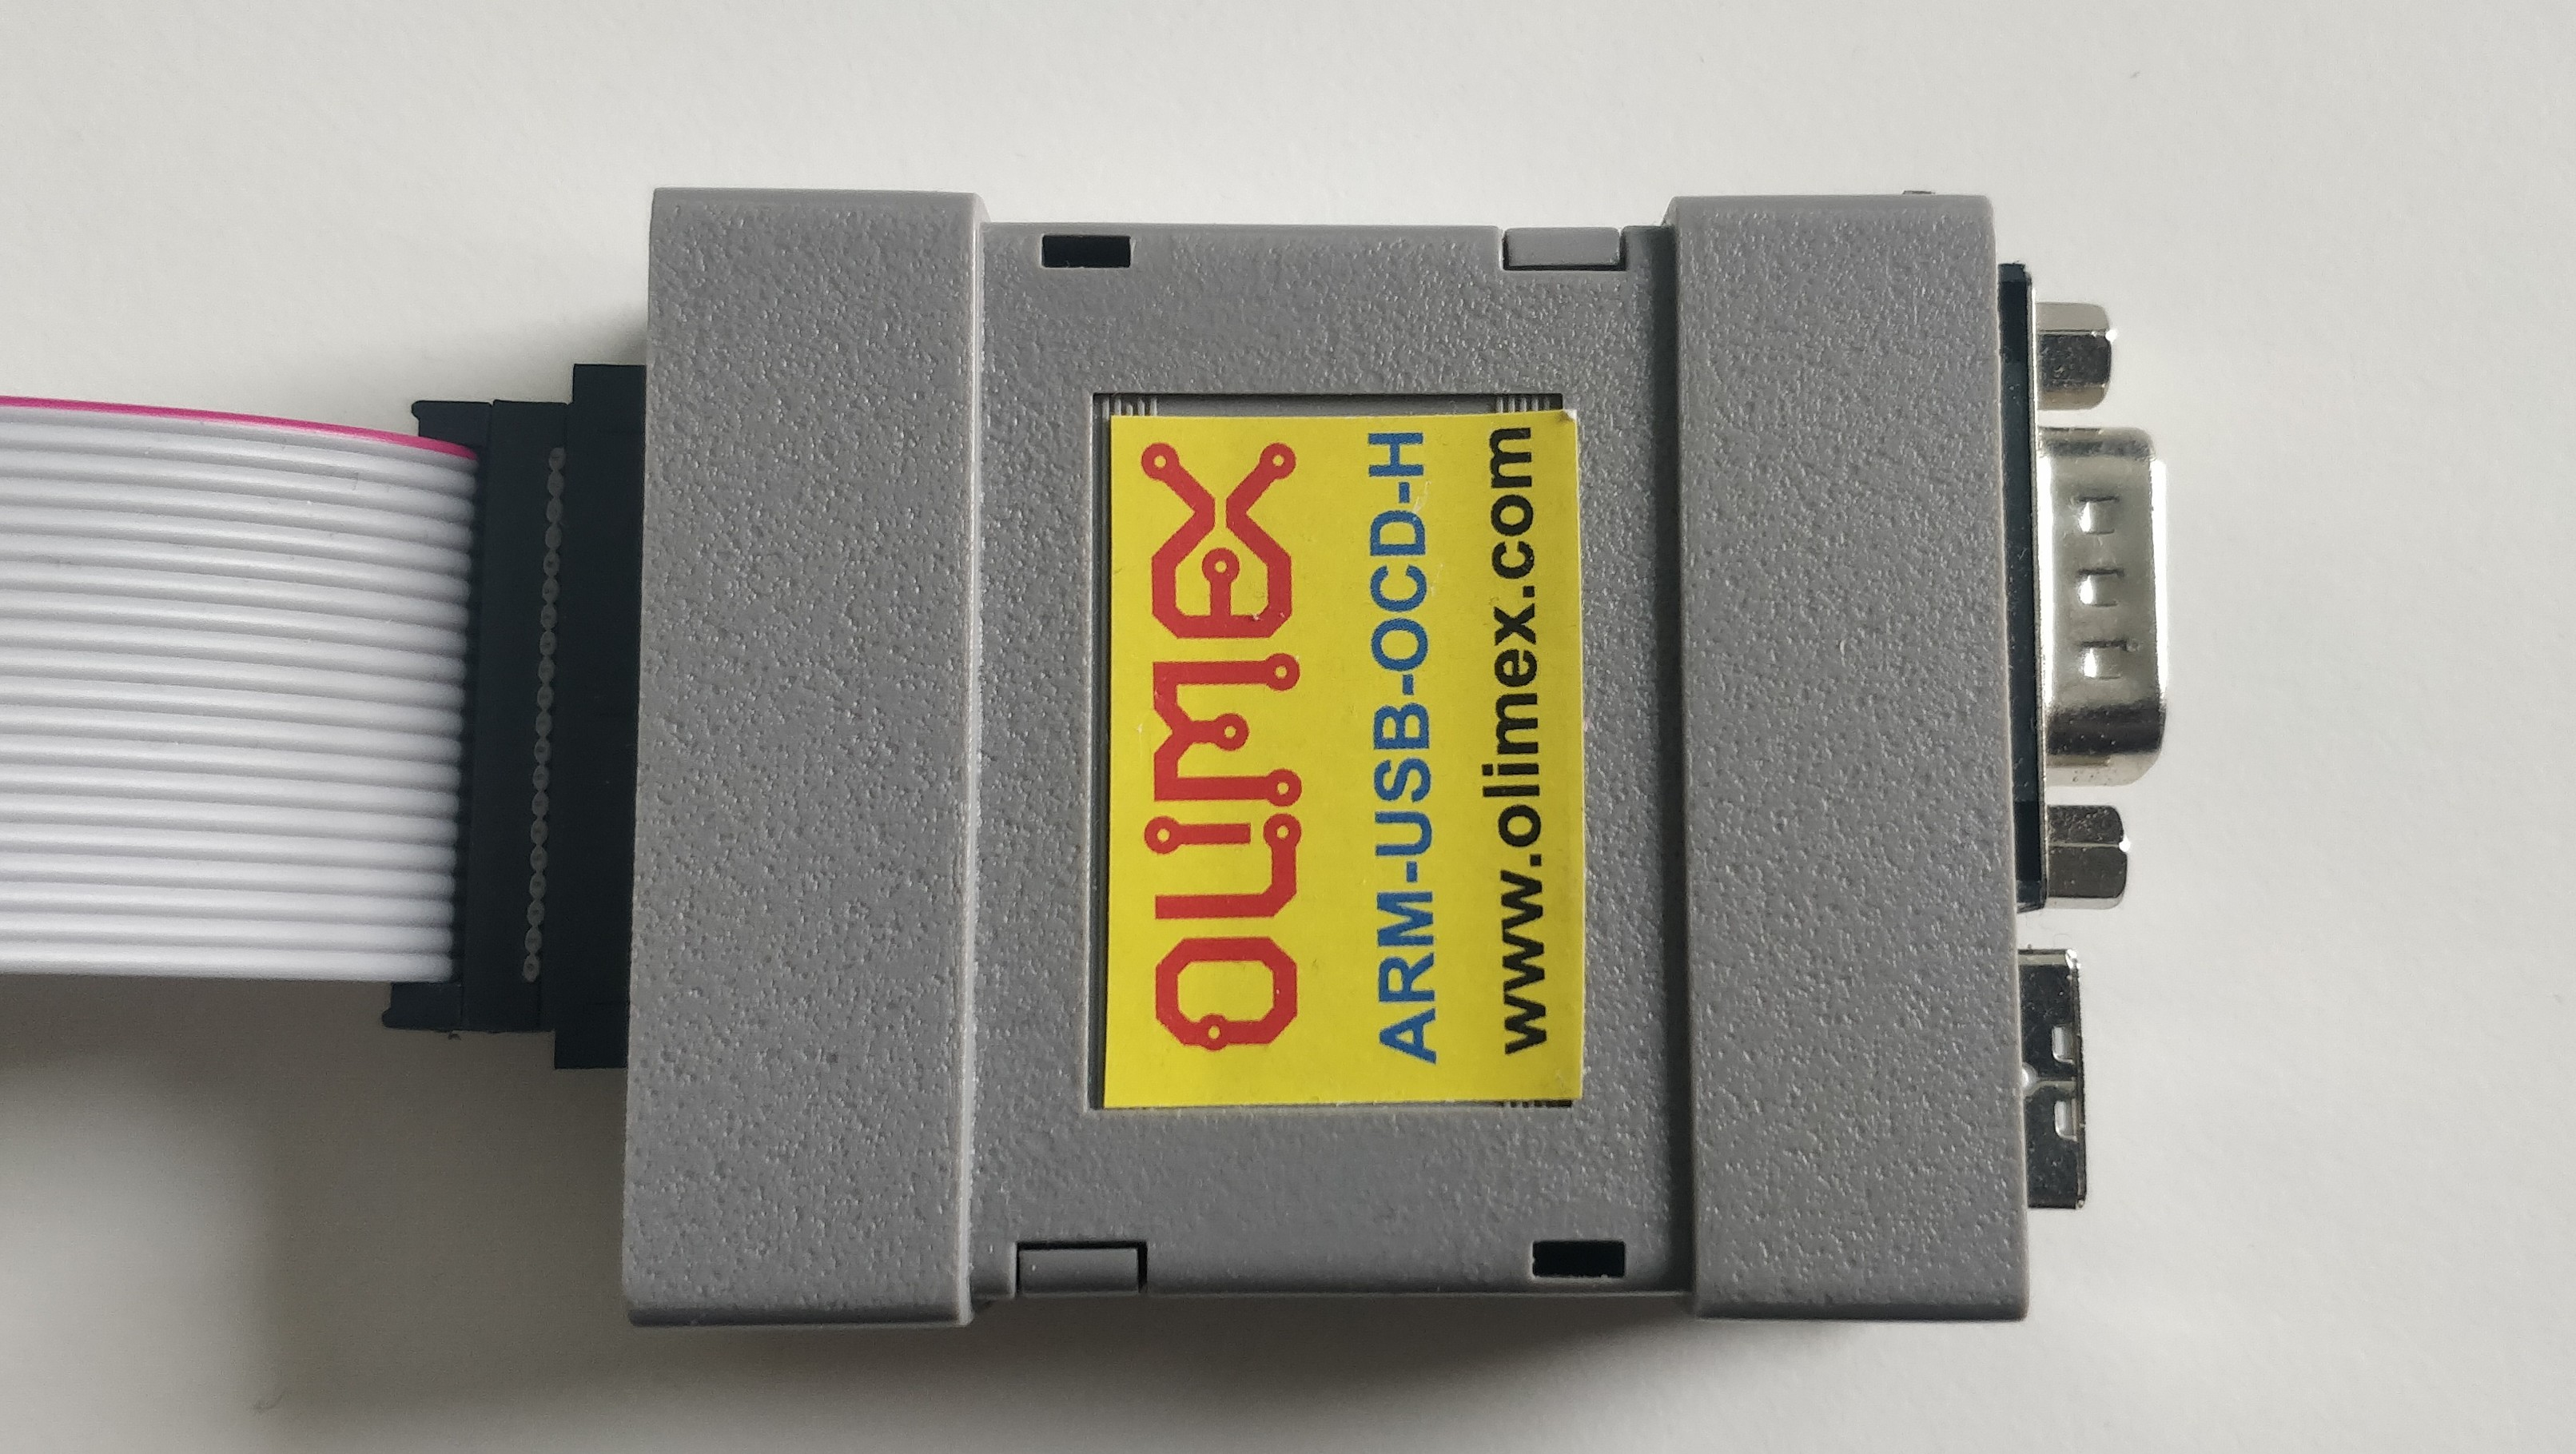
\includegraphics[scale=0.05]{fig/jtagusbocd.jpg}

\captionof{figure}[Olimex-stm32-e407 with Debugger]{Olimex-stm32-e407 with Debugger}
\label{fig:jtag}
\end{center}
\item The configuration to enable micro-ROS examples, self-made publisher and subscriber with BMP180 pressure sensor, and also the delay test algorithm can be found in my repository. 

To connect the pressure sensor with the board (you might need the help of the board's datasheet, see link - \href{https://www.olimex.com/Products/ARM/ST/STM32-E407/resources/STM32-E407.pdf}{Olimex-stm32-e407 datasheet}\cite{olimexdatasheet}), we need 4 UART cables and then connect them in the following sequence :
				\begin{center}
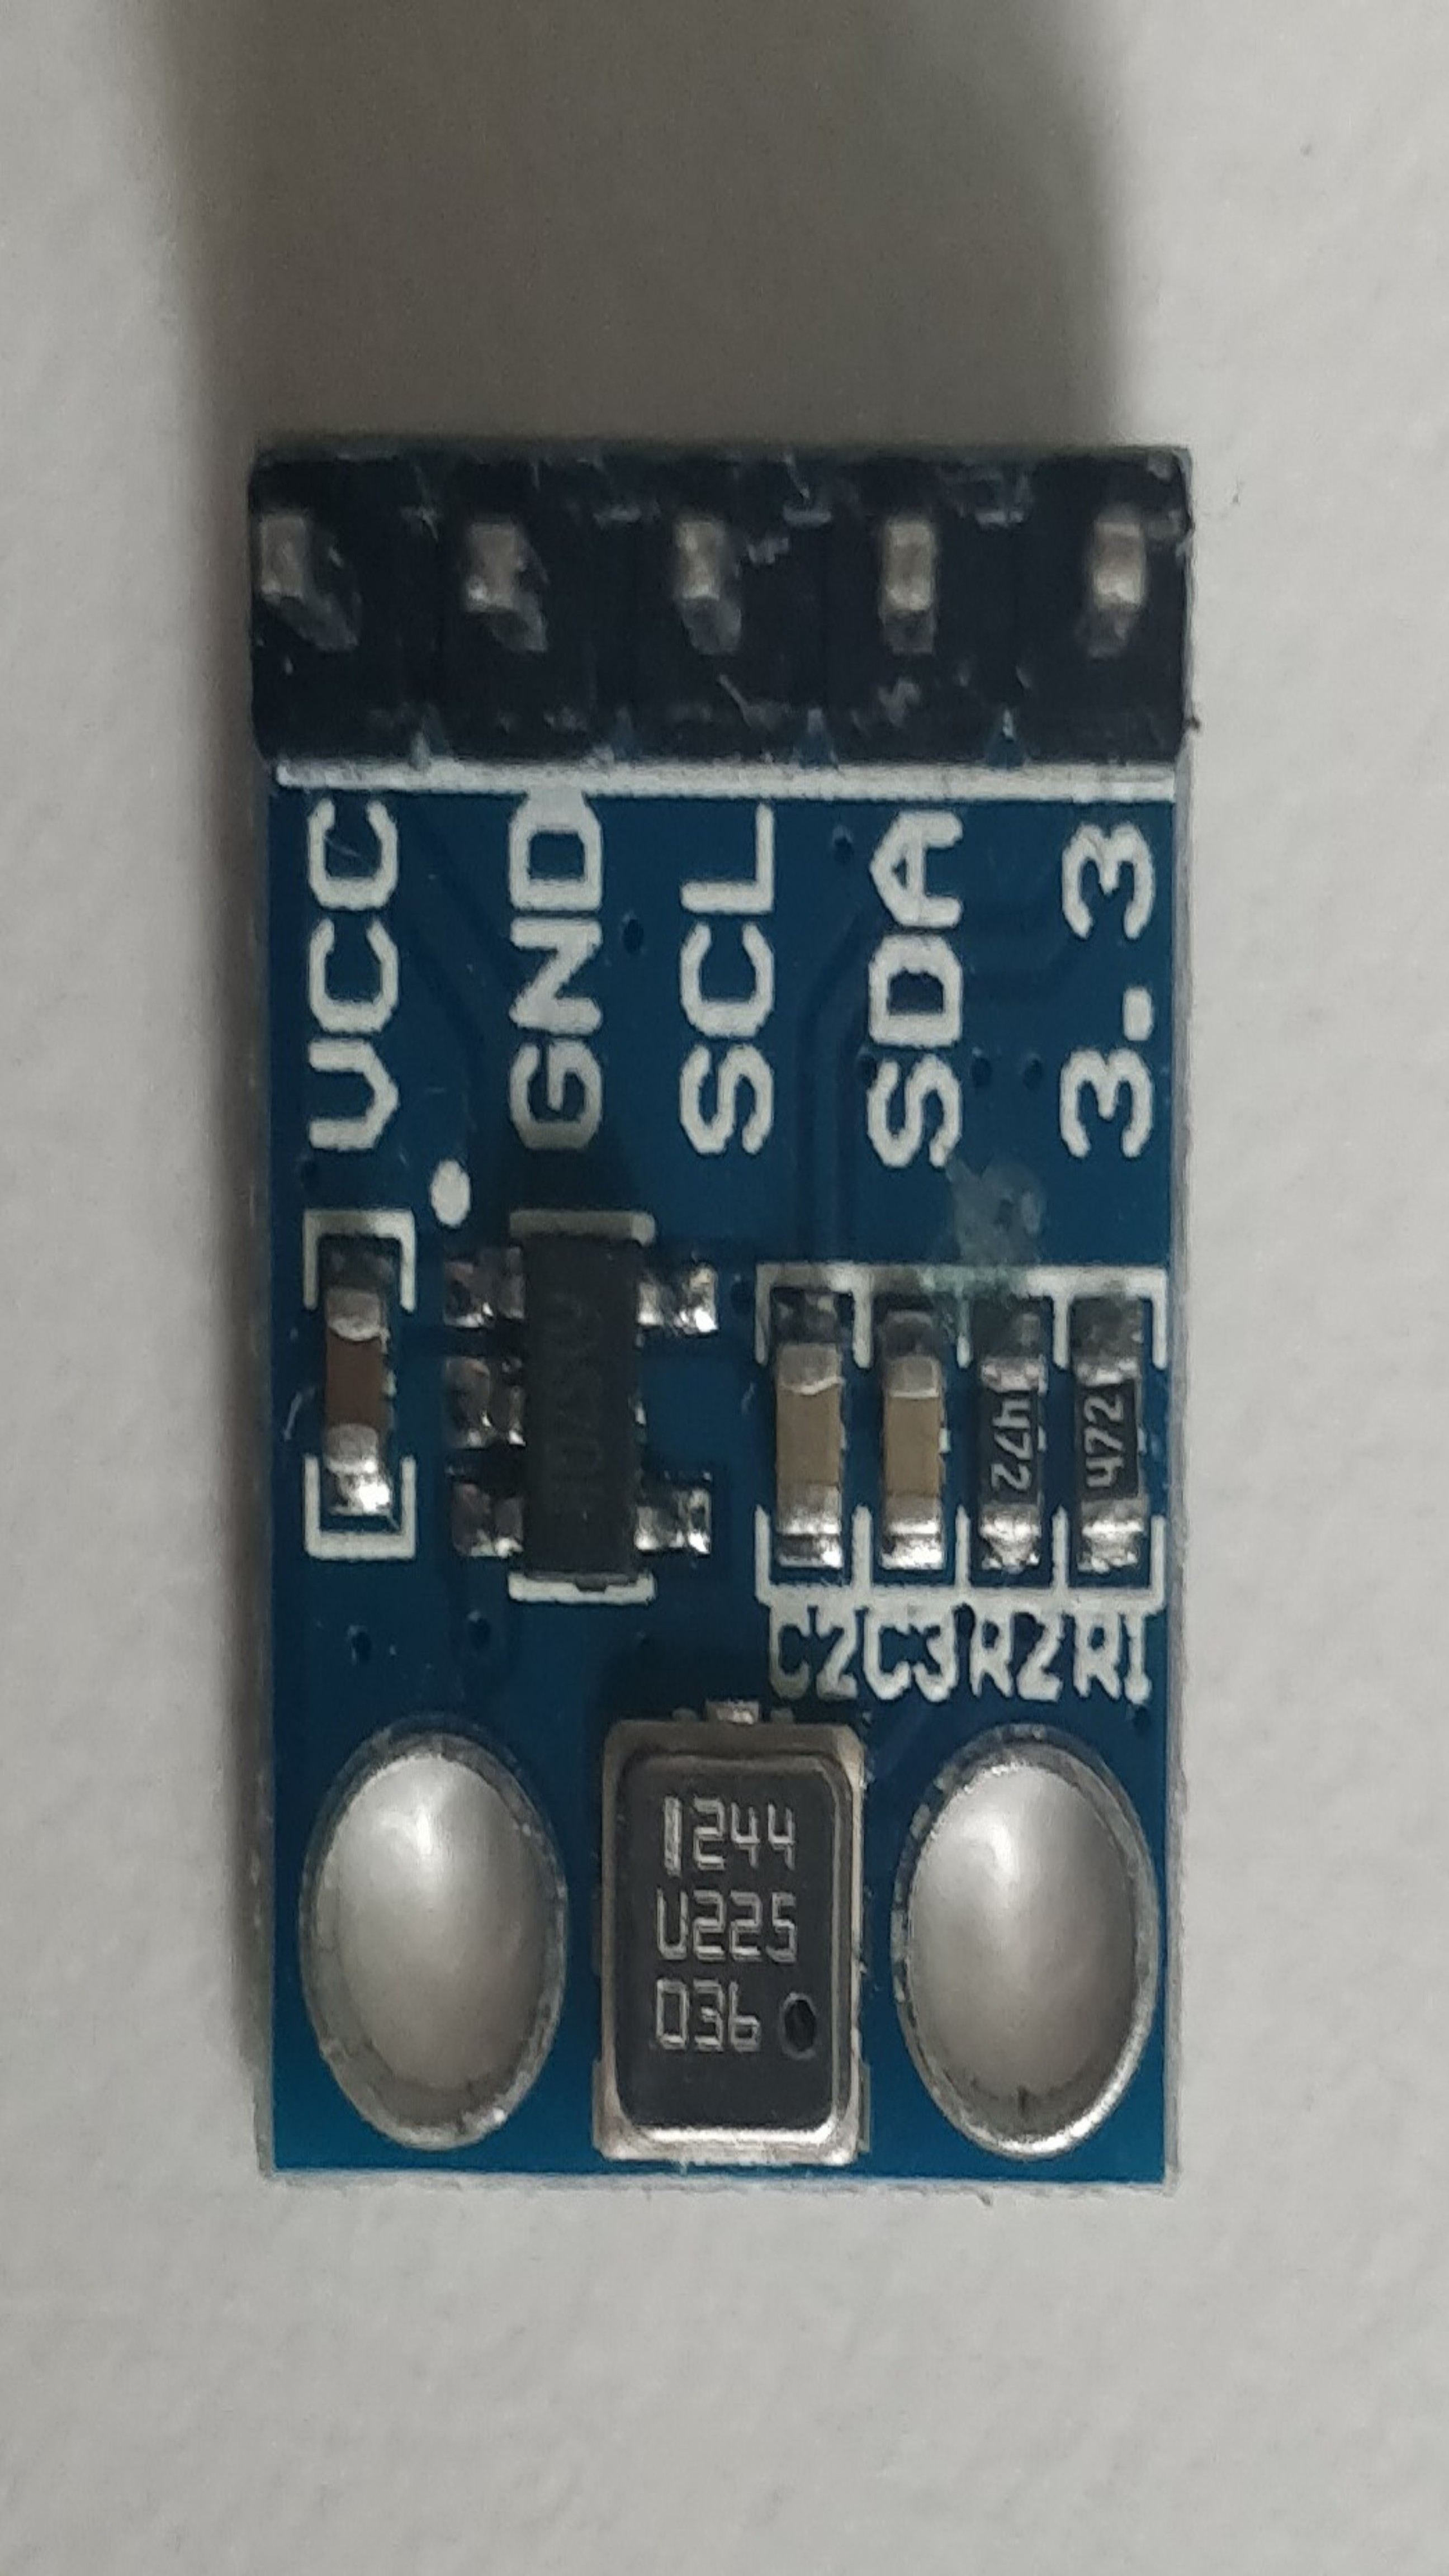
\includegraphics[scale=0.03,angle=270]{fig/pressuresensor.jpg}

\captionof{figure}[BMP180 Pressure Sensor]{BMP180 Pressure Sensor}
\label{fig:bmp180}
\end{center}
\begin{itemize}
\item Connect Vcc to board's 3V(volts) terminal.
\item Connect GND to board's Ground terminal.
\item Connect SCL to board's DO terminal.
\item Connect SDA to board's D1 terminal.
\end{itemize}

\item Connect the ethernet wire to the socket. After flashing is complete, press the reset button and open a terminal in your Linux computer. Type "dmesg" to check the USB port to which the board is connected.
\item Then type "sudo minicom -s" and select the USB port and enter your password. Once minicom launches, press enter 3 times. Nuttx console will be seen in the terminal.
\item Type "ifup eth0" to enable ethernet. Type "ifconfig" to check IP addresses of the device and network. Then type "mount -t procfs proc" to mount the file system to access the network applications.
\item Type "help" to see all built-in applications. You should be able to see publisher, subscriber, bmp180\textunderscore publisher, bmp180\textunderscore subscriber, and delay\textunderscore test.
\item The delay\textunderscore test adds a timestamp, then publishes a message and sends to the agent and subscribes it back again. Then it adds another timestamp and calculates the difference between the initial time and final time. Hence, we have the delay in micro-ROS communications.
\begin{center}
\hspace*{-1cm}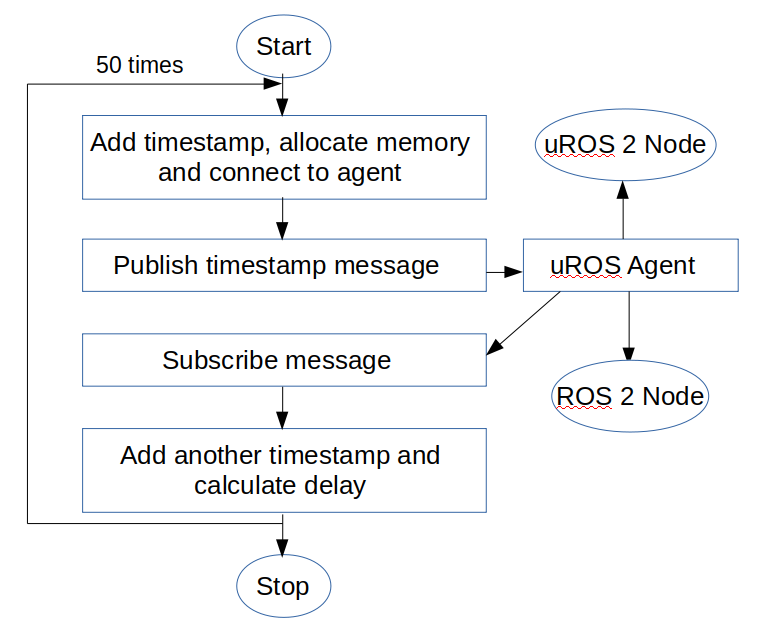
\includegraphics[scale=0.3]{fig/delay.png}

\captionof{figure}[Delay Test]{Delay Test}
\label{fig:delay}
\end{center}
\item To increase the data sizes of the messages, custom ROS messages were created and testing was repeated with message sizes of 8 bytes (an integer data size is 4 bytes), 16 bytes, 32 bytes,64 bytes and 128 bytes.
\begin{center}
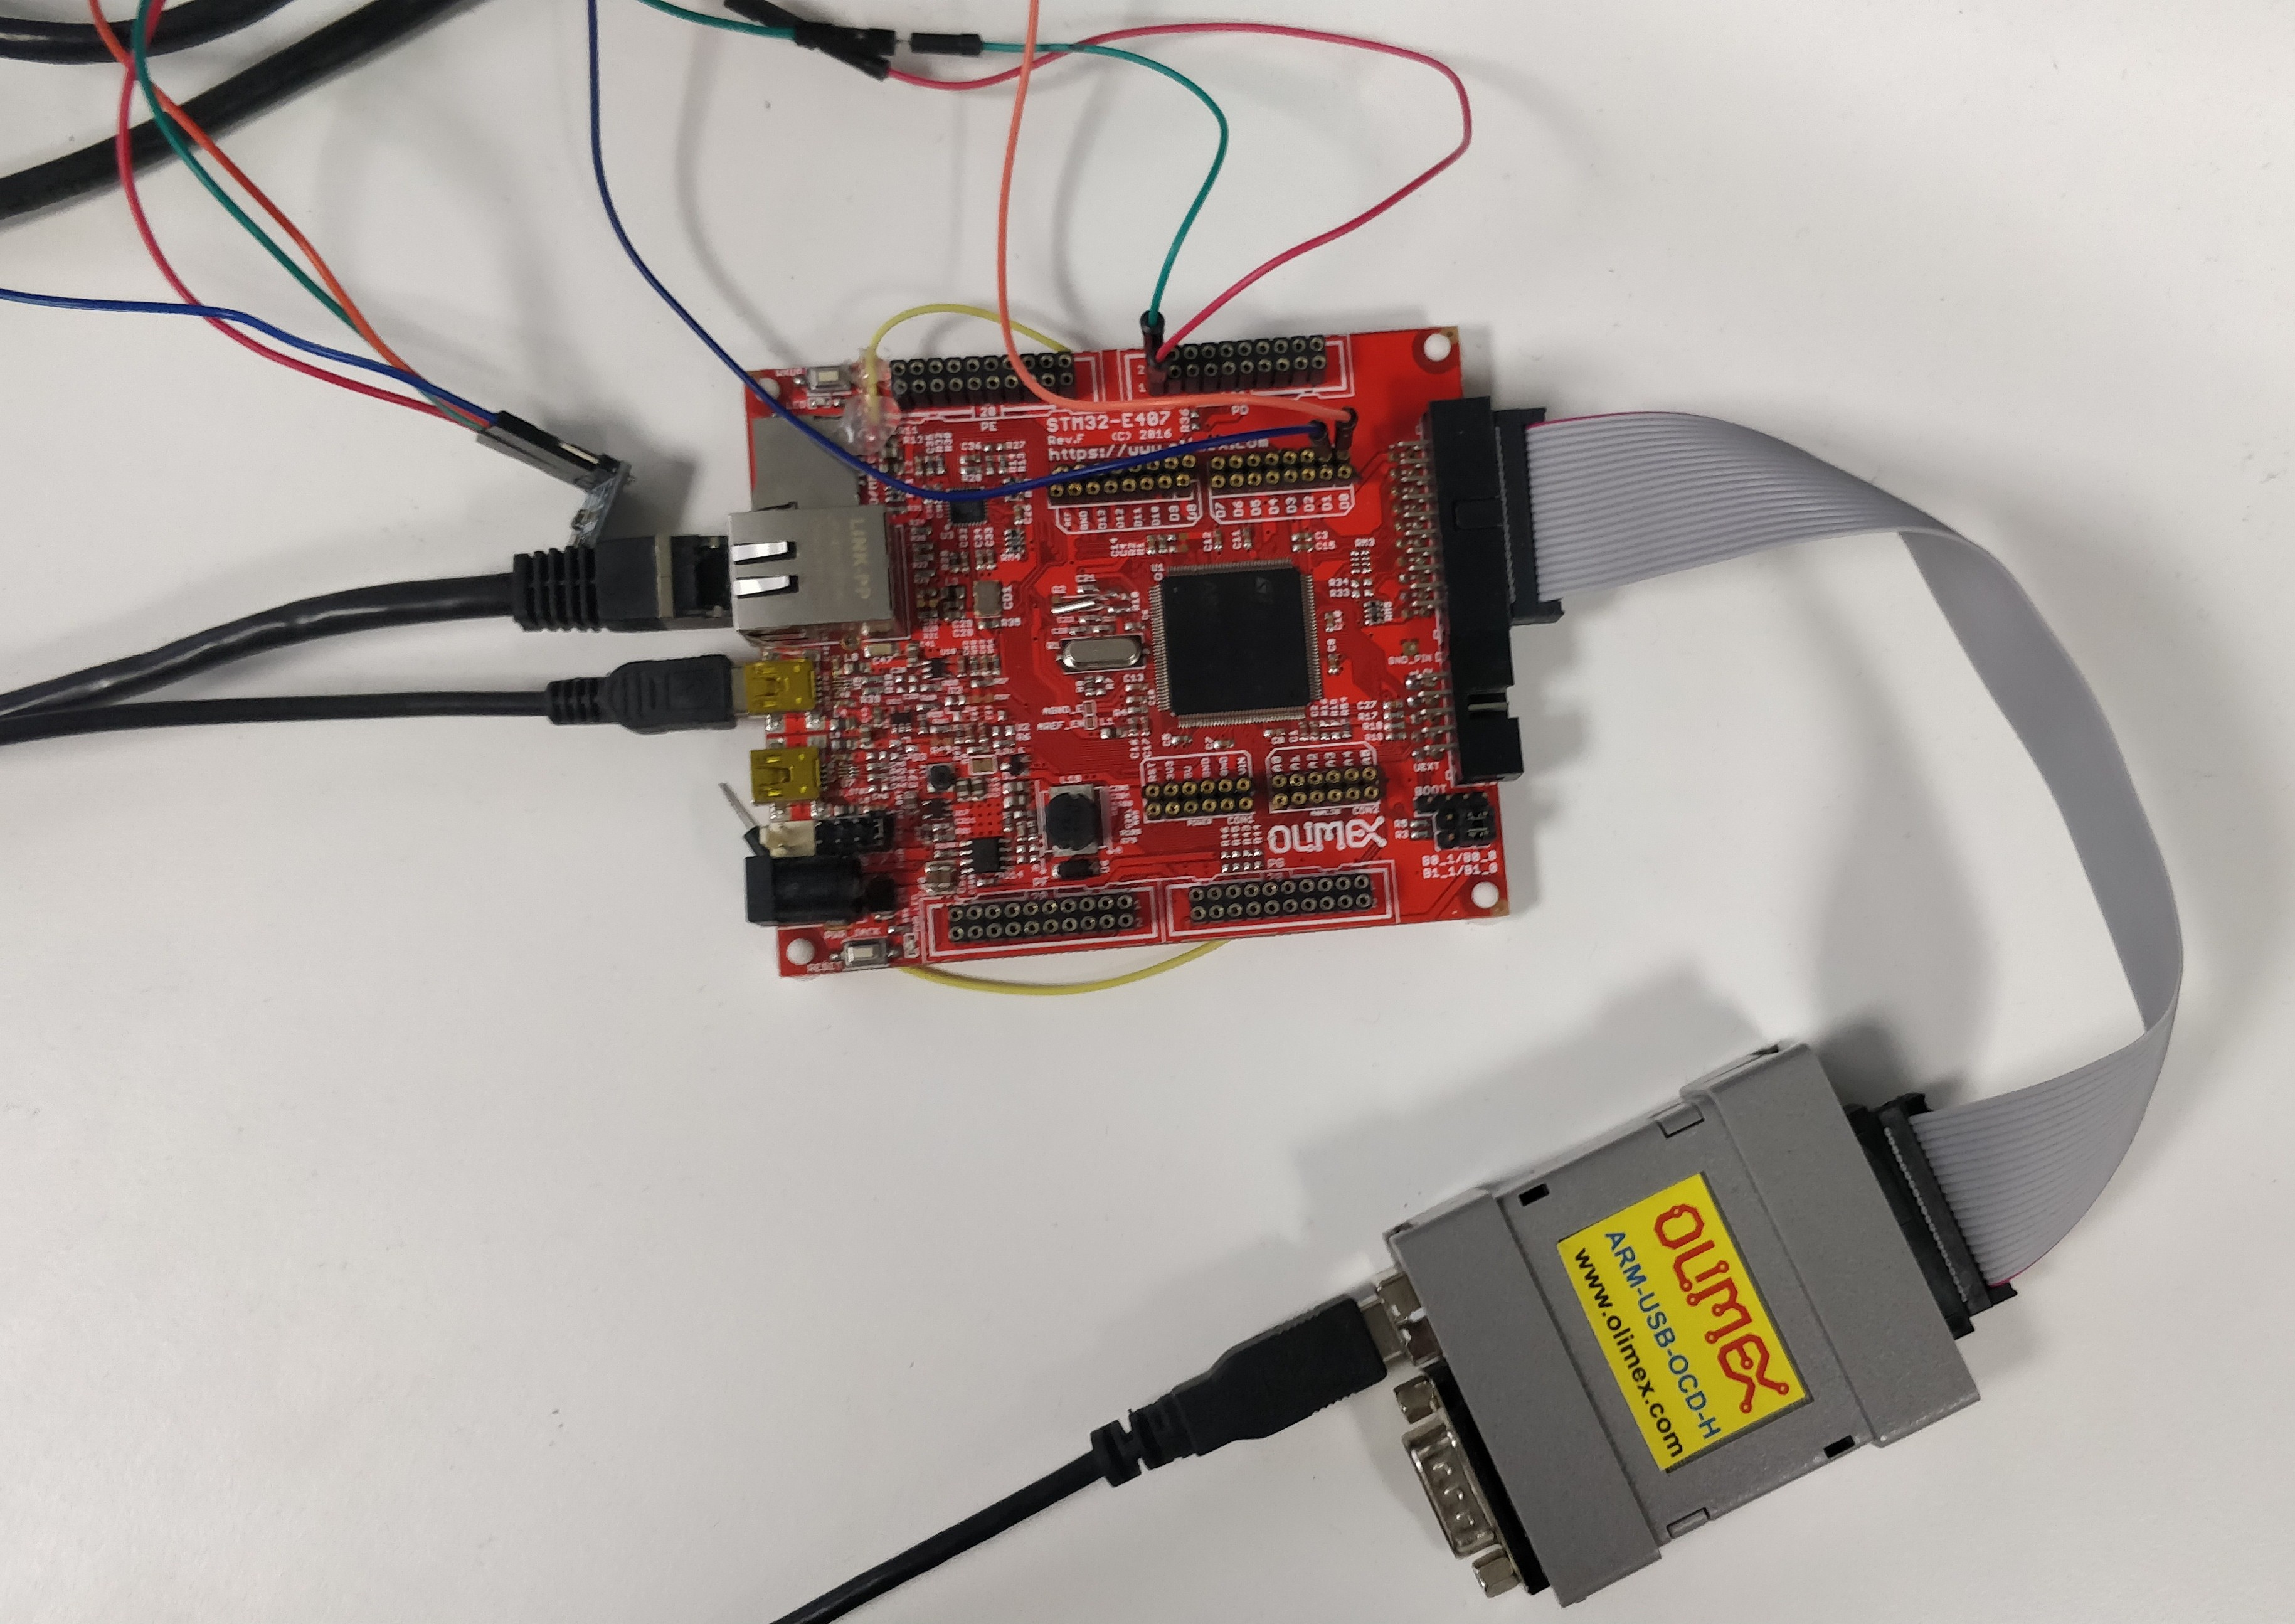
\includegraphics[scale=0.1]{fig/olimex.jpg}

\captionof{figure}[Olimex Setup]{Olimex Setup}
\label{fig:olimexsetup}
\end{center}
\item Similarly, set up the waveshare board. Skip steps 5 and 8 as we don't need pressure sensor and ethernet connection. Although, if required, DP83848 ethernet to UART converter can be used to setup ethernet as well. We will connect a USB to UART converter cable to enable serial transport of micro-ROS. To do this connect the wires as shown : 
\begin{itemize}
\item Black wire of connector to ground of the board using UART3 port
\item Green wire to RX port.
\item White wire to TX port.
\end{itemize}
\item Launch the micro-ROS Agent in another terminal in Linux. First source the ROS 2 crystal environment, then source the micro-ROS environment. Then go to the micro-ROS agent package in the install directory and launch micro-ROS agent with commands "./micro\textunderscore ros\textunderscore agent udp 8888" for IP connection and "./micro\textunderscore ros\textunderscore agent serial <USB port number for PL2303 driver>". Then launch the delay\textunderscore test application in Nuttx. delay\textunderscore test was done 50*10 times using a loop and all data was recorded
\end{enumerate}
\begin{center}
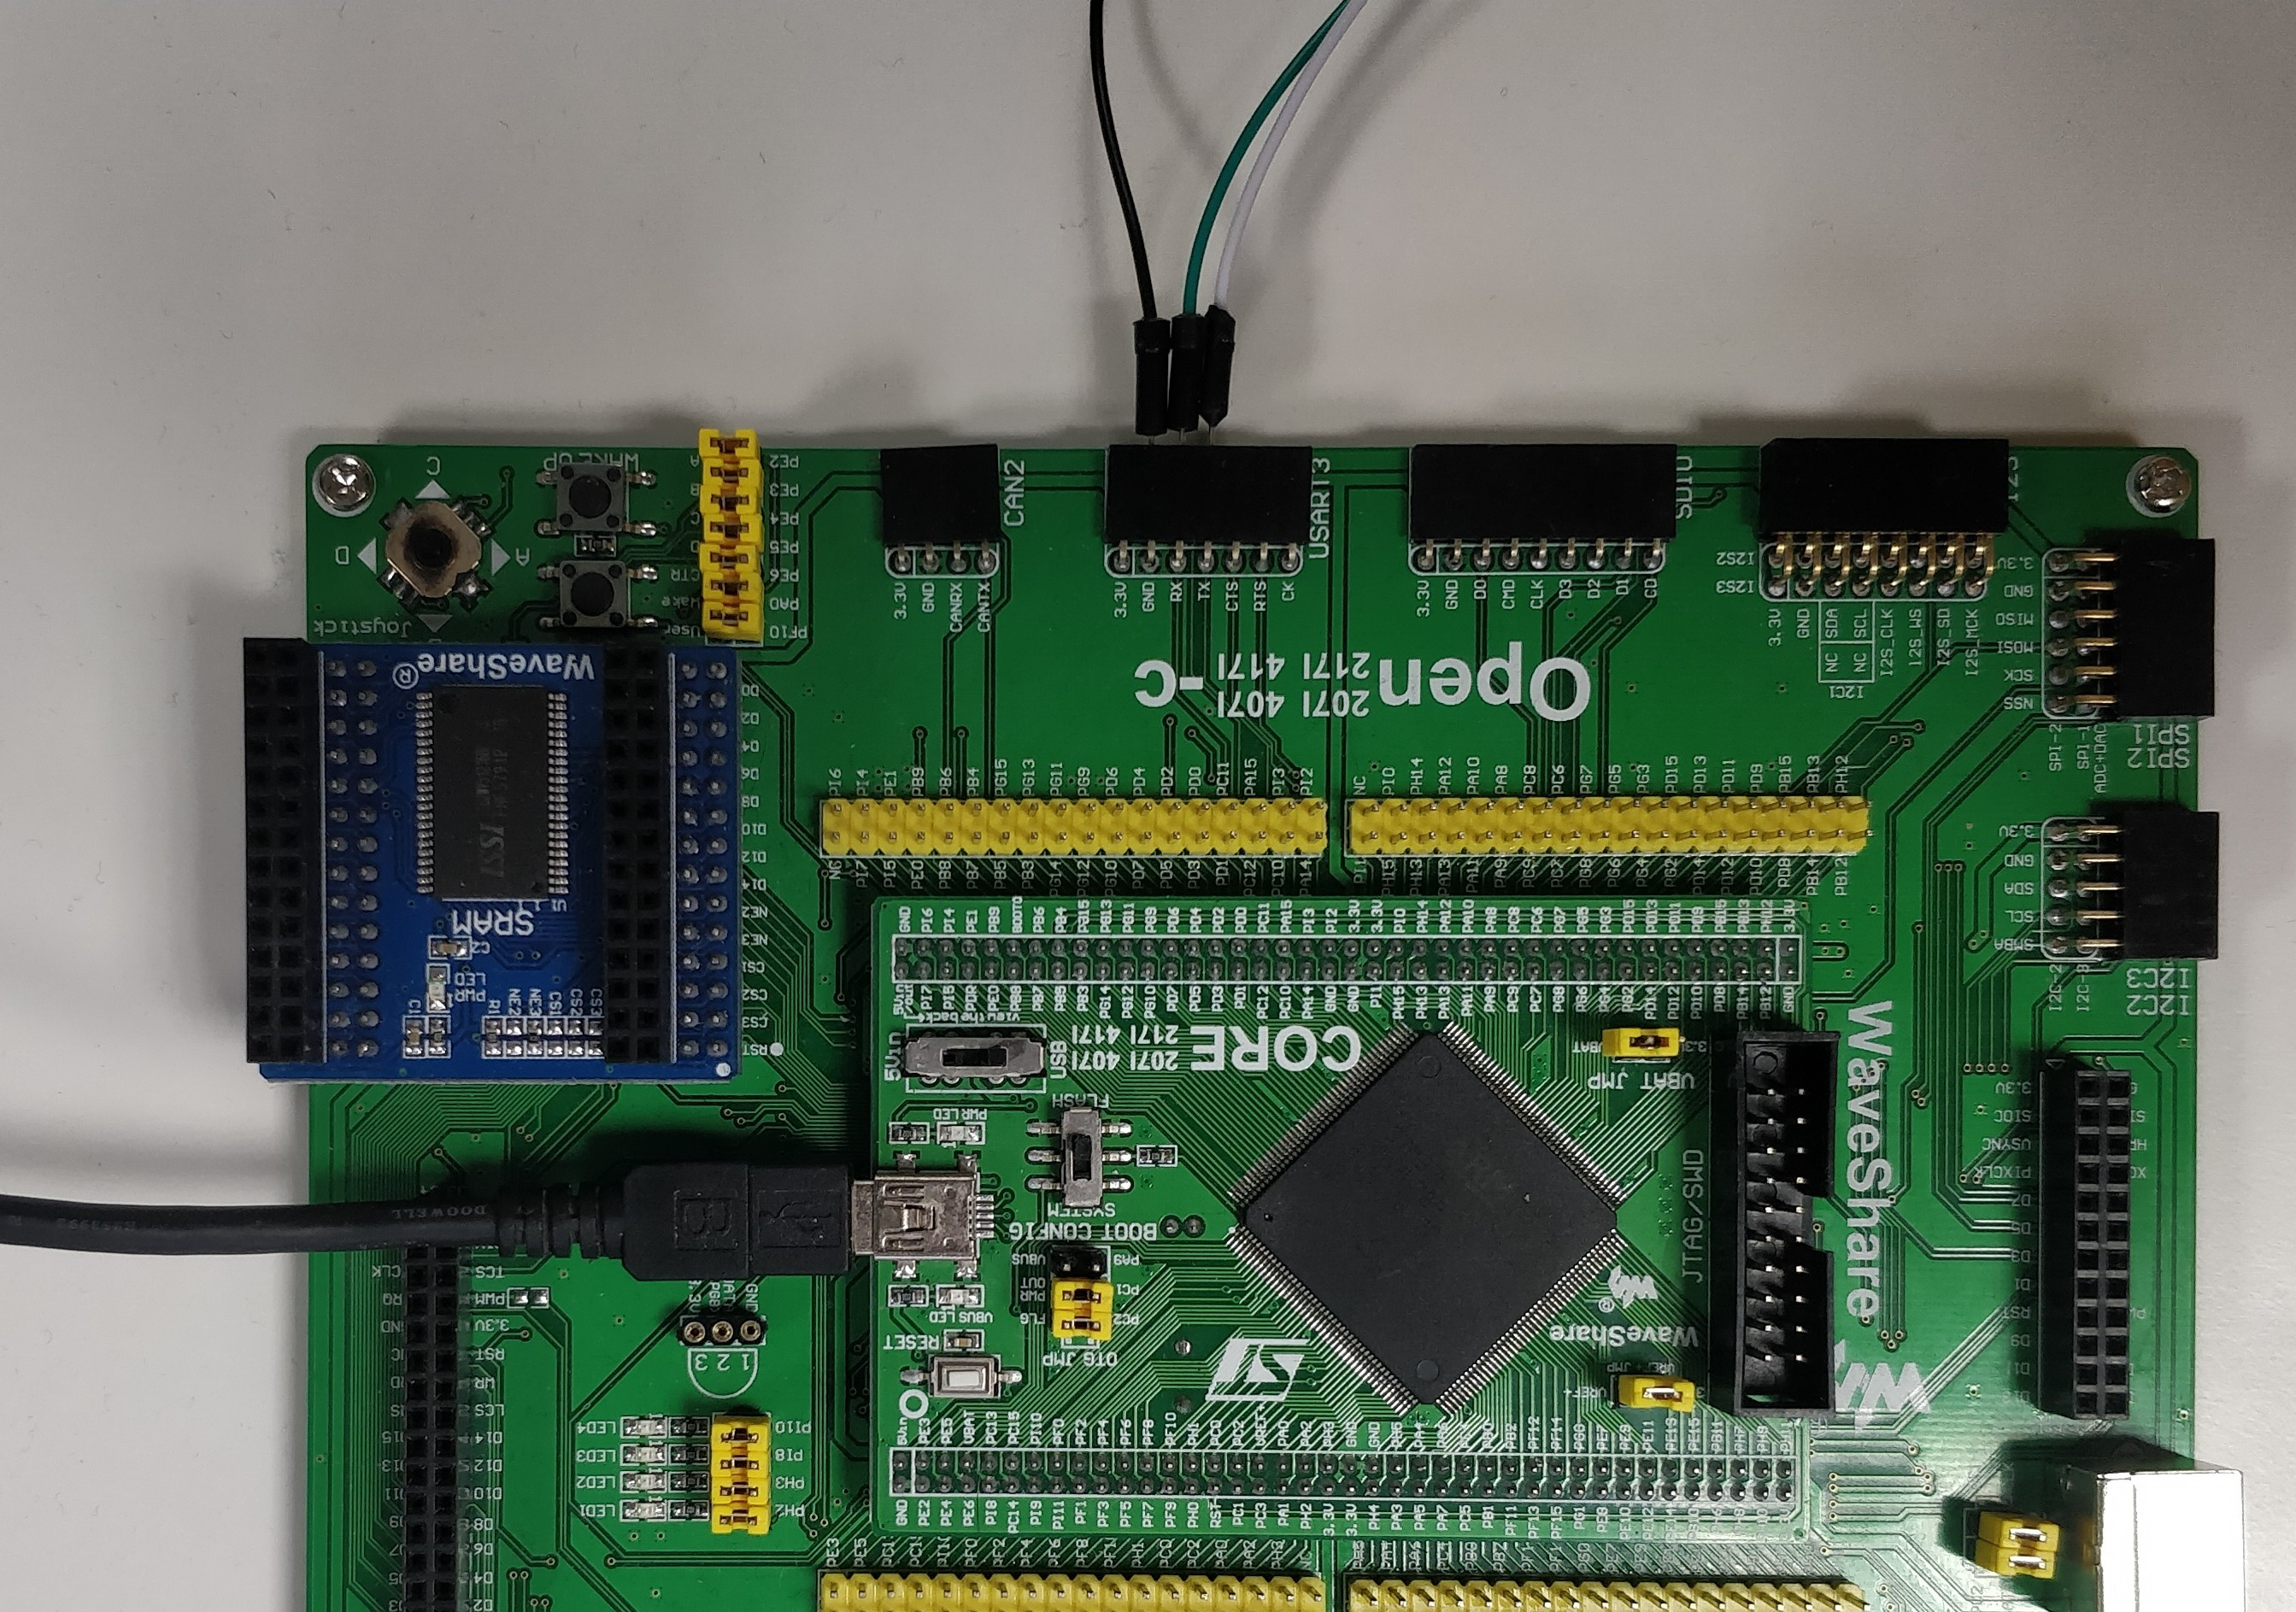
\includegraphics[scale=0.15,angle=180]{fig/waveshare.jpg}

\captionof{figure}[Waveshare Setup]{Waveshare Setup}
\label{fig:wavesharesetup}
\end{center}
		\chapter{Results}
			
\rofoot[\pagemark]{\pagemark}
\refoot[\pagemark]{\pagemark}
		
		\section{Latency Analysis of ROS 2}
\vspace*{0.5cm}
{\bfseries ROS 2 Crystal}
\begin{center}
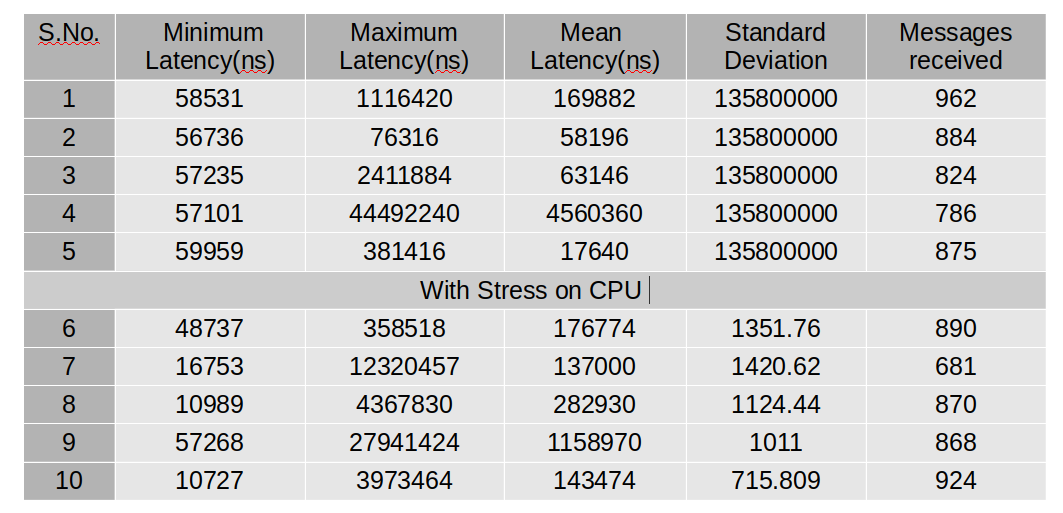
\includegraphics[scale=0.4]{fig/ros2crylatency.png}

\captionof{table}[ROS 2 Crystal Latency]{ROS 2 Crystal Latency}
\label{tab:ros2crystallatency}
\end{center}
In this package, the messages are sent every 1 ms. The goal of this package was to receive 1000 messages with maximum 3\% jitter(30 us). In this testing, 1 MB of memory and high real-time priority is available to the node. The package is not reliable as we can see we lose messages. Even though we have low latency values, still we can see the mean latency over 1 ms in 2 observations which is greater than the update rate. The maximum latency is 44.5 ms. We also see very high standard deviation values which suggests the software is not deterministic even without any stress on the CPU. The maximum jitter value is 33 ms which is way beyond the desired.
\vspace*{0.5cm}


{\bfseries ROS 2 Dashing}
\vspace*{0.5cm}

In this package, the messages are sent every 1 ms. In this testing, 1 MB of memory and high real-time priority is available to the node. The jitter and standard deviation keep on increasing with time. The maximum jitter value is 80 ms but the package defines the deadline as 2 ms. Although, the mean jitter value close to zero and the pendulum not falling down suggests firm real-time performance but the increasing standard deviation and high jitter values give us an impression that some improvements in the ROS 2 execution is required to make ROS 2 hard real-time. It should also be taken into consideration that the Linux real-time kernel does not guarantee a hard real-time system.
\begin{center}
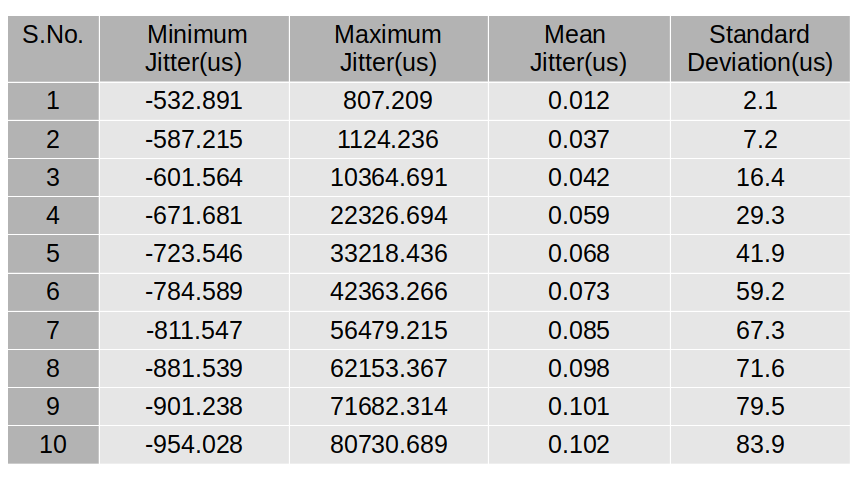
\includegraphics[scale=0.4]{fig/ros2dashjitter.png}

\captionof{table}[ROS 2 Dashing Jitter]{ROS 2 Dashing Jitter}
\label{tab:ros2dashjit}
\end{center}
		\section{Reliabilty of micro-ROS}
		\vspace*{0.5cm}
		Some software bugs and missing features were found during the testing:
	\begin{itemize}	
	\item Multiple microcontrollers can not be connected to a single micro-ROS Agent/Server. This is one of the important features of micro-ROS which is missing. The issue has been reported to the developers.
\begin{itemize}
\item {\bfseries Case 1} : Using built-in publisher-subscriber of micro-ROS through ethernet (UDP) with one micro-ROS Agent. 
Publisher was launched on the olimex board and subscriber was launched on the waveshare board. Both of them were communicating through the same IP address and port number. Message sending rate is really fast (1ms) in this example, subscriber code was changed to receive 500 messages and then stop. \linebreak
{\bfseries Result} : Only one of the nodes work, either publisher or subscriber.

\item {\bfseries Case 2} : Using built-in publisher-subscriber of micro-ROS through ethernet (UDP) with two micro-ROS Agents with different port numbers.\linebreak
{\bfseries Result} : same as above

\item {\bfseries Case 3} : Using bmp180 pressure sensor and same structure of publisher-subscriber code as the built-in example through ethernet(UDP), first with one micro-ROS Agent and then 2 Agents with different port number.
Message is sent every 1 second.\linebreak
{\bfseries Result} : Both nodes are initialised at both the boards. Subscriber receives very less data, for instance, it receives only 2 messages while the publisher publishes 15 messages in the same time, therefore it is not reliable.

\item {\bfseries Case 4} : Built in publisher-subscriber with 1 Agent through ethernet (UDP) and 1 Agent through serial (UART) communication.
Data sending rate is 1 ms.\linebreak
{\bfseries Results} : Nodes are initialised, but many messages are not received by the subscriber, therefore it is not reliable.

\item {\bfseries Case 5} : Using BMP180 pressure sensor with 1 Agent through ethernet (UDP) and 1 Agent through serial (UART) communication.
Data is sent every 1 second. \linebreak
{\bfseries Results} : Nodes are initialised and all values are received.
\end{itemize}
\item Arrays are not supported in the messages. Therefore, strings messages or array of numbers or an image can not be transported as of now. Therefore, I had to use a pressure sensor to use the standard integer message package. Also, testing of large message sizes could not take place.

\end{itemize}
\section{Latency Analysis of micro-ROS}
\vspace*{0.5cm}
In this testing of delay in micro-ROS communications, sometimes the subscriber got timed out and killed the node which hampered testing. Later, it was confirmed with the developers that this is also a bug in the software. Due to this issue, multiple publishers and subscribers present in a single node could not be tested. Also the latencies using the UART serial communication were 15-20 ms more than the latencies using ethernet (UDP) communication because of the lag caused by the driver in the USB to UART converter. Therefore further testing was only done using ethernet. We have some promising results :
\begin{itemize}
\item Below, you can see the latencies in nanoseconds for 500 observations for a message size of 8 bytes. The least count of the board's clock was 10 ms.

\begin{center}
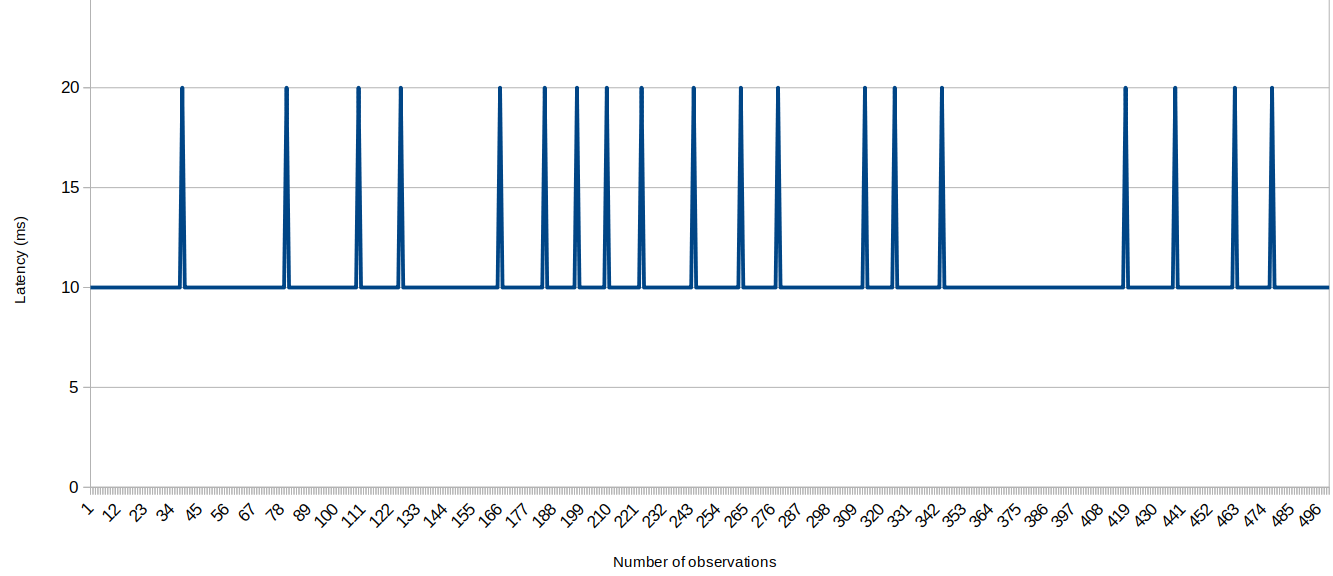
\includegraphics[scale=0.3]{fig/uros8byteles.png}
\captionof{figure}[Micro-ROS Latencies for Data Size of 8 bytes (Least count-10 ms)]{Micro-ROS Latencies for Data Size of 8 bytes (Least count-10 ms)}
\label{fig:uros8byteles}
\end{center}

\item Below, you can see the latencies in nanoseconds for 500 observations for a message size of 8 bytes. The least count of the board's clock was changed to 10 us for better precision. This is followed by the observations of the delay test with message size of 16 bytes, 32 bytes, 64 bytes and 128 bytes.
\nomenclature{MB}{Megabyte}
\nomenclature{ns}{Nanoseconds}
\nomenclature{ms}{Milliseconds}
\nomenclature{us}{Microseconds}
\begin{center}
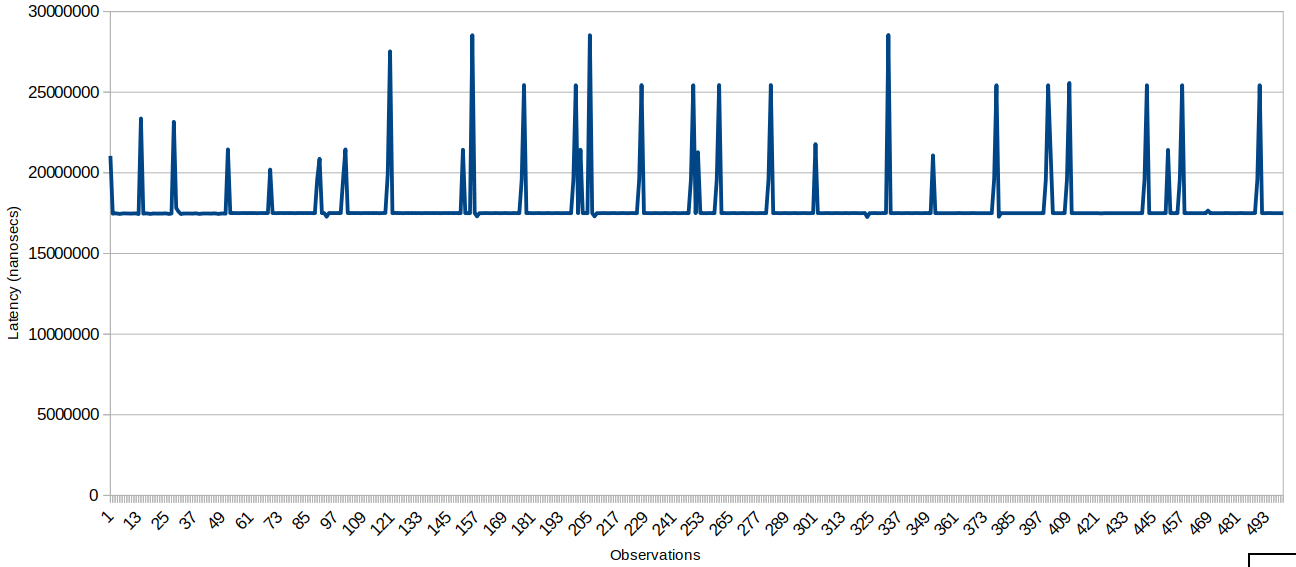
\includegraphics[scale=0.32]{fig/uros8byte.png}

\captionof{figure}[Micro-ROS Latencies for Data Size of 8 bytes (Least count-10 us)]{Micro-ROS Latencies for Data Size of 8 bytes (Least count-10 us)}
\label{fig:uros8byte}
\end{center}


\begin{center}
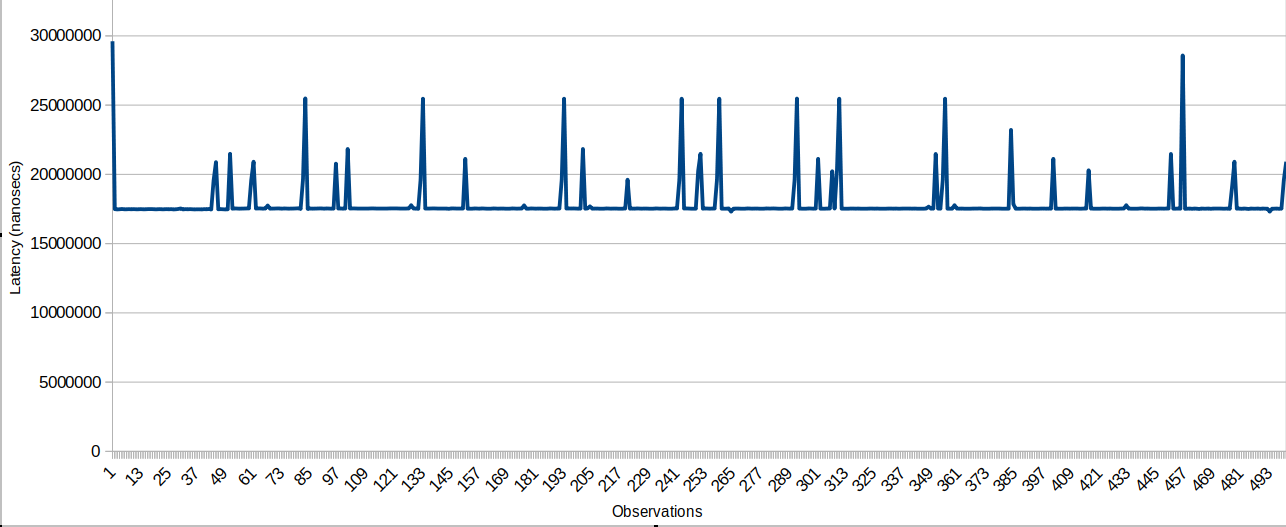
\includegraphics[scale=0.32]{fig/uros16byte.png}

\captionof{figure}[Micro-ROS Latencies for Data Size of 16 bytes (Least count-10 us)]{Micro-ROS Latencies for Data Size of 16 bytes (Least count-10 us)}
\label{fig:uros16byte}
\end{center}

\begin{center}
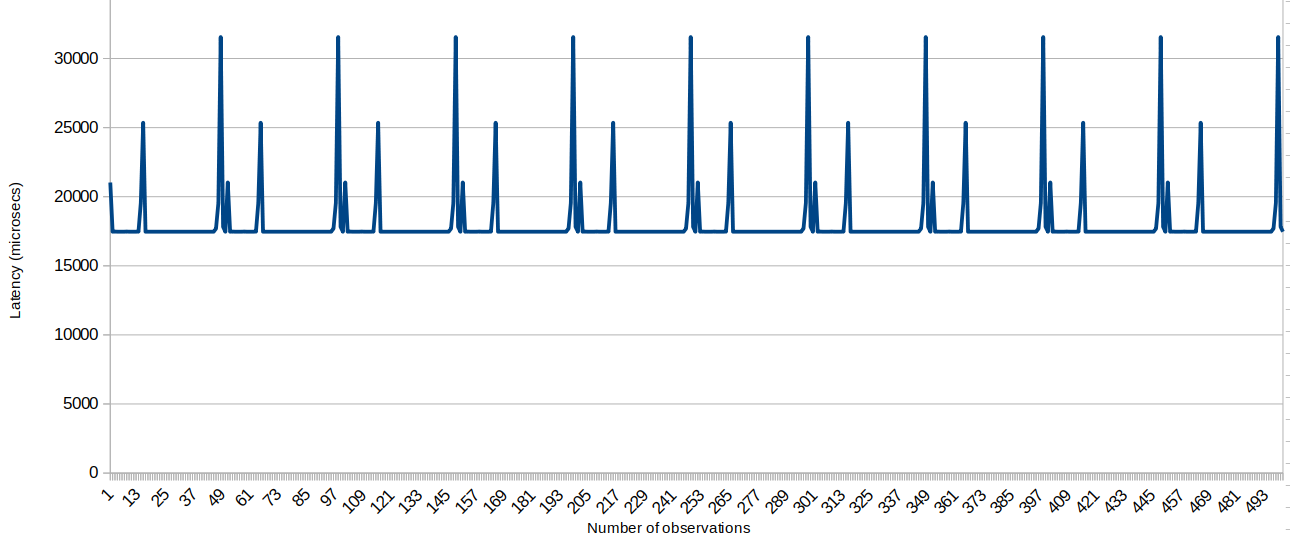
\includegraphics[scale=0.32]{fig/uros32byte.png}

\captionof{figure}[Micro-ROS Latencies for Data Size of 32 bytes (Least count-10 us)]{Micro-ROS Latencies for Data Size of 32 bytes (Least count-10 us)}
\label{fig:uros32byte}
\end{center}

\begin{center}
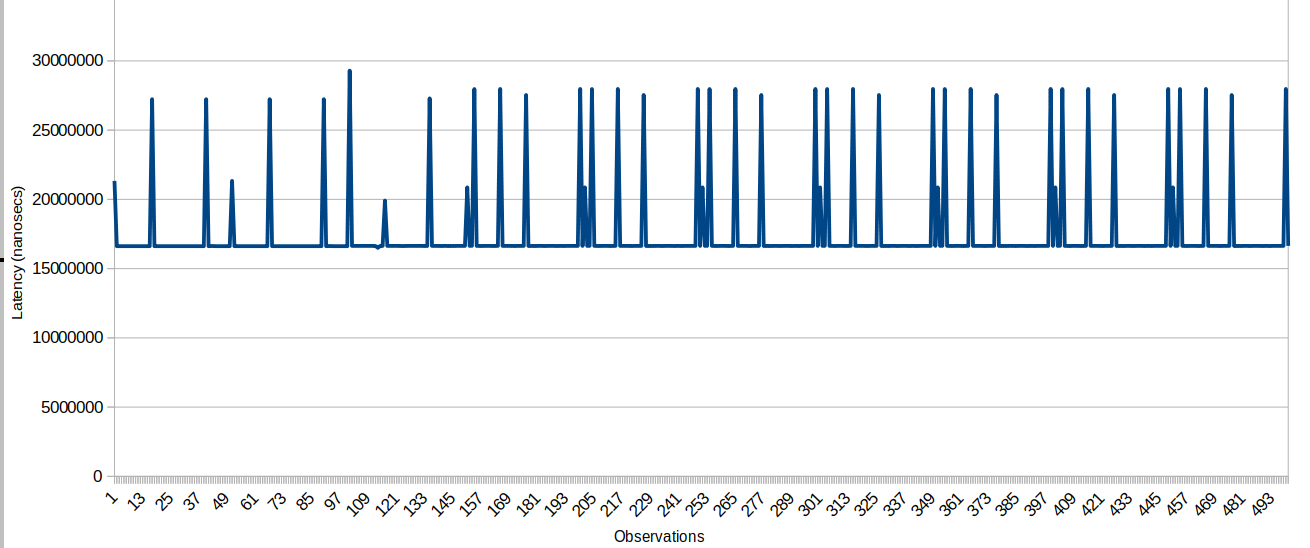
\includegraphics[scale=0.32]{fig/uros64byte.png}

\captionof{figure}[Micro-ROS Latencies for Data Size of 64 bytes (Least count-10 us)]{Micro-ROS Latencies for Data Size of 64 bytes (Least count-10 us)}
\label{fig:uros64byte}
\end{center}

\begin{center}
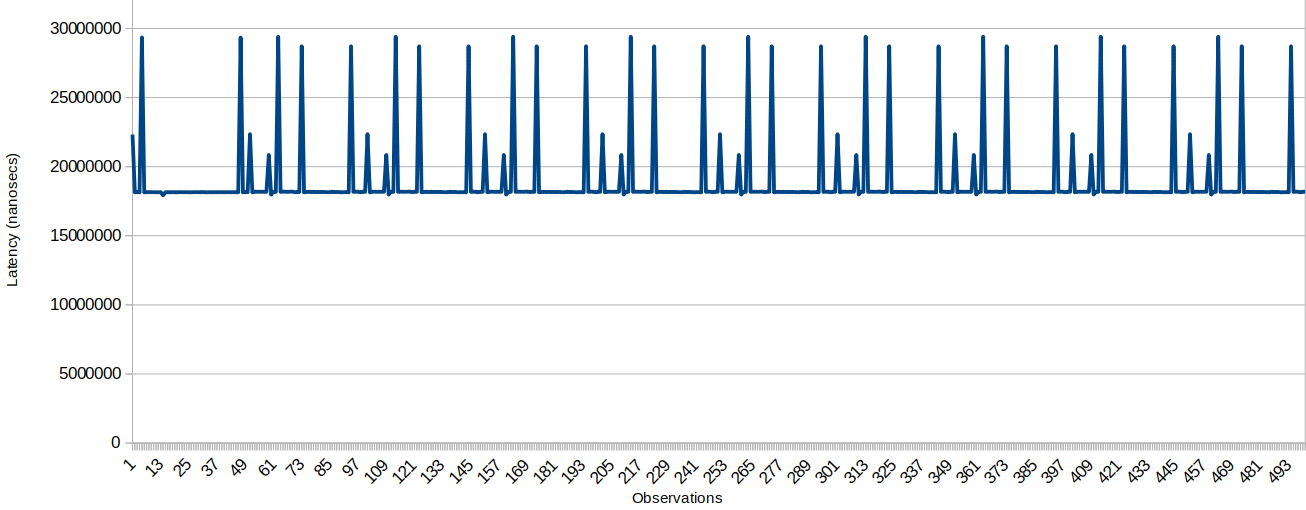
\includegraphics[scale=0.32]{fig/uros128byte.png}

\captionof{figure}[Micro-ROS Latencies for Data Size of 128 bytes (Least count-10 us)]{Micro-ROS Latencies for Data Size of 128 bytes (Least count-10 us)}
\label{fig:uros128byte}
\end{center}
\end{itemize}
{\bfseries Analysis}


\vspace*{0.5cm}
From the line graphs, we can see the deterministic performance of the micro-ROS LET Executor. Let us define an acceptable jitter value of 1 ms. A large number of latency spikes outside the range of acceptable jitter were observed. Below, in the table we can find the summary of observations. We can see low mean jitter values which suggests good real-time performance with a RTOS. Also, we can observe that the number of observations with excessive jitter increase with the message size.
\begin{center}
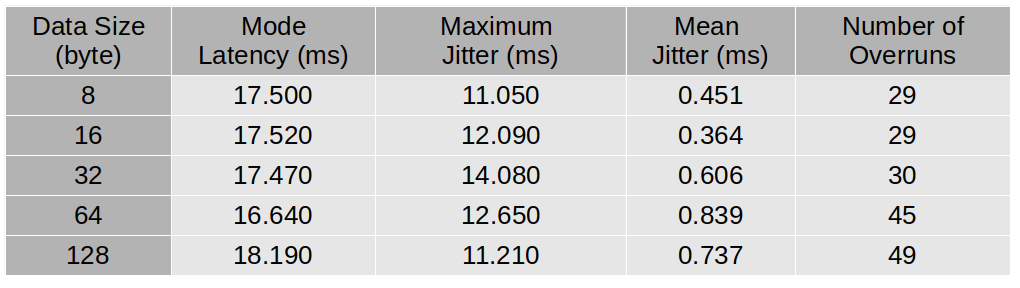
\includegraphics[scale=0.4]{fig/urosfinaldata.png}

\captionof{table}[Micro-ROS Results]{Micro-ROS Results}
\label{tab:urosfinaldata}
\end{center}
		
		\section{Discussion and Comparison}
		\vspace*{0.25cm}
	Since, the packages and ways of testing for ROS 2 Crystal, ROS 2 Dashing and micro-ROS (ROS 2 Crystal) are different. The results should not be compared between them. However, we can still determine some common aspects of their results.
	
	ROS 2 Crytal pendulum demo is a broken simulation and does not show good real-time performance. The mean latencies values are low but the large standard deviation and maximum latencies are not good for a real-time system. Also, there is loss of data which increases when stress is applied. This package does not exactly help in testing real-time capabilities.
	\vspace*{0.25cm}
	
	ROS 2 Dashing pendulum demo provides more accurate results and also offers a continuous visual simulation in RViz. Mean jitter values are very low but they keep on icreasing with time. Also the high maximum jitter and standard deviation values suggests there is some improvement needed to make the execution more deterministic. It also gives us an impression that with some fine-tuning and improvements in the ROS 2 Standard Executor, the software can be configured for a soft or firm real-time system. Development of real-time systems with the standard ROS 2 stack and Linux environment requires a lot of research work and ROS 2 package development at this moment. However, with a RTOS and proper real-time code structure, ROS 2 can offer better real-time performance. Real-time applications with the standard ROS 2 stack can not be seen in the ROS 2 Community, but the main issues related to real-time performance have been identified and the community is working along with ROS 2 developers to improve the real-time performance of ROS 2.
	
	\vspace*{0.25cm}
	There is also an alternative to the standard ROS 2, which is micro-ROS specifically targeting embedded board and real-time applications. However, extensive development of micro-ROS is required to provide a reliable software without bugs and missing features. The C++ Executor is still a challenge as many applications in the robotic world use C++. The testing of this software was partially successful. We observed the deterministic behavior of the LET Executor and low mean jitter values. But we also observed high maximum jitter values. Even though, micro-ROS runs on a RTOS, the Agent still requires a Linux environment which is not real-time safe. The Agent is a core element of the communication structure and running it on a non RTOS will have a negative impact on the real-time performance of micro-ROS. Also, multiple number of publishers and subscribers could not be launched due to a software bug and stress could not be applied to the microprocessor.
		\chapter{Conclusion}
			
\rofoot[\pagemark]{\pagemark}
\refoot[\pagemark]{\pagemark}
Our investigations in the real-time performance of the standard ROS 2 stack suggest that it is a good software for automotive applications and gives promising initial results but still requires improvements and further development in some of its packages to make it suitable for a real-time system, especially hard real-time applications. We also need to use a RTOS and configure it to be real-time safe. Currently, it only seems suitable for soft real-time systems. Also, the underlying DDS middleware can be fine-tuned for better real-time performance, but this needs to be further investigated. Based on the ROS community discussions, the issues with the software have been identified and we might see some special features related to real-time systems in the upcoming versions of ROS 2. The inverted pendulum demo can be used as a standard platform to test the upcoming versions.

\vspace*{0.5cm}
micro-ROS offers deterministic behavior and seems more suitable than the standard ROS 2 stack for a real-time system. But, it requires extensive and fast development to offer its users a real-time safe and reliable software. Still the limitations of this software remain to be tested as there are a lot of bugs and their development needs to integrate with the standard ROS 2 stack. Also, the micro-ROS Agent dependency needs to be eliminated because it runs on an environment which is not real-time safe.


\section{Future Scope}
\vspace*{0.5cm}
\begin{itemize}
\item Future versions of ROS 2 can be tested with the inverted pendulum demo and the results can be compared with that of Dashing.
\item Research on configuration and fine tuning of DDS by different vendors for better real-time performance. 
\item Testing of inverted pendulum demo with micro-ROS and RTOS when the C++ Executor becomes available.
\item Real-time testing of image messages using a camera sensor and micro-ROS as image processing is of interest for the development of automated driving.
\item Develop a physical hardware setup of an inverted pendulum for testing with micro-ROS.
\item Compare ROS 2 with other softwares in the same testing environment. For example, the Driverless Formula Student Racing Team at the Ravensburg Weingarten University can compare the performance of softwares with brake distance or lap time.
\end{itemize}
		\addcontentsline{toc}{chapter}{List of Figures}
	\listoffigures
	\addcontentsline{toc}{chapter}{List of Tables}
	\listoftables
		
		\addcontentsline{toc}{chapter}{Bibliography}
\bibliographystyle{ieeetr}		
\bibliography{thesis}





\end{document}
